\chapter{Étude de la méthode}
    \label{chapter:4-ETUDES}
	
	% RÉSUMÉ DES ÉPISODES PRÉCÉDENTES:
	Dans le chapitre précédent, nous avons présenté une méthode de création d'un jeu de données d'entrainement pour un assistant conversationnel, que nous appelons "\textit{clustering interactif}" :
	%
	\begin{todolist}
	    % 1. Structure de la méthode.
		\item[\itemok] La méthode proposée repose sur la combinaison entre un regroupement automatique des données par la machine et l'annotation de contraintes binaires par un expert métier pour corriger le regroupement proposé ;
		% 2. Enjeu 1 de la méthode : moins de technique.
		\item[\itemok] Une telle approche devrait limiter les pré-requis techniques actuellement exigés à un expert métier en les déléguant à la machine.
		% 2. Enjeu 2 de la méthode : plus de connaissance métier.
		\item[\itemok] En échange, l'expert se concentre d'avantage sur la transmission de ses connaissances avec une annotation caractérisant la similitude métier entre deux données.
		% 3. Divers.
		\item[\itemok] ...\todo{divers à compléter (technique ? méthode ? ...).}
	\end{todolist}
	
	% ANNONCE DU BUT DU CHAPITRE: TEST DE LA MÉTHODE.
	Comme nous l'avons détaillé dans le chapitre~\ref{chapter:2-ETAT-DE-L-ART}, des procédés d'annotation similaires existent pour des données facilement visualisables, comme dans le cadre du traitement d'images. Cependant, l'application d'une telle approche dans le cadre de la classification de données textuelles est peu détaillée dans la littérature. Ainsi, dans cette partie, nous étudierons la faisabilité d'un \textit{clustering interactif} pour des données textuelles en explorant les questions suivantes :
	%
	\begin{todolist}
		% 1. Efficacité.
		\item Peut-on obtenir une base d'apprentissage à l'aide de notre proposition d'implémentation de la méthodologie d'\textit{clustering} interactif ? (cf. hypothèse d'\textbf{efficacité} en section~\ref{section:4.1-HYPOTHESE-EFFICACITE})
		% 2. Efficience.
		\item Peut-on déterminer un paramétrage optimal de cette implémentation pour obtenir plus rapidement une base d'apprentissage ? (cf. hypothèse d'\textbf{efficience} en section~\ref{section:4.2-HYPOTHESE-EFFICIENCE})
		% 3. Pertinence.
		\item A un instant donné, peut-on estimer la pertinence métier d'une base d'apprentissage en cours de construction ? (cf. hypothèse de \textbf{pertinence} en section~\ref{section:4.3-HYPOTHESE-PERTINENCE})
		% 4. Coûts.
		\item D'après les données initiales, peut-on approximer l'investissement nécessaire pour obtenir une base d'apprentissage exploitable ? (cf. hypothèse sur les \textbf{coûts} en section~\ref{section:4.4-HYPOTHESE-COUTS})
		% 5. Impact.
		\item A un instant donné, peut-on estimer les gains potentiels d'une nouvelle étape de raffinage de la base d'apprentissage en cours de construction ? (cf. hypothèse d'\textbf{impact} en section~\ref{section:4.5-HYPOTHESE-IMPACT})
		% 6. Robustesse.
		\item Peut-on estimer l'influence d'une erreur ou d'une différence d'annotation dans la construction de la base d'apprentissage ? (cf. hypothèse de \textbf{robustesse} en section~\ref{section:4.6-HYPOTHESE-ROBUSTESSE})
	\end{todolist}
	
	% ILLUSTRATION: SCHEMA DES HYPOTHESES
	Afin d'illustrer ces interrogations, nous vous proposons de considérer de la figure~\ref{figure:HYPOTHESE-00-DEFAULT}. Dans les sections suivantes, cette figure évoluera pour résumer les études réalisées.
	%
	\begin{figure}[H]
		\centering
		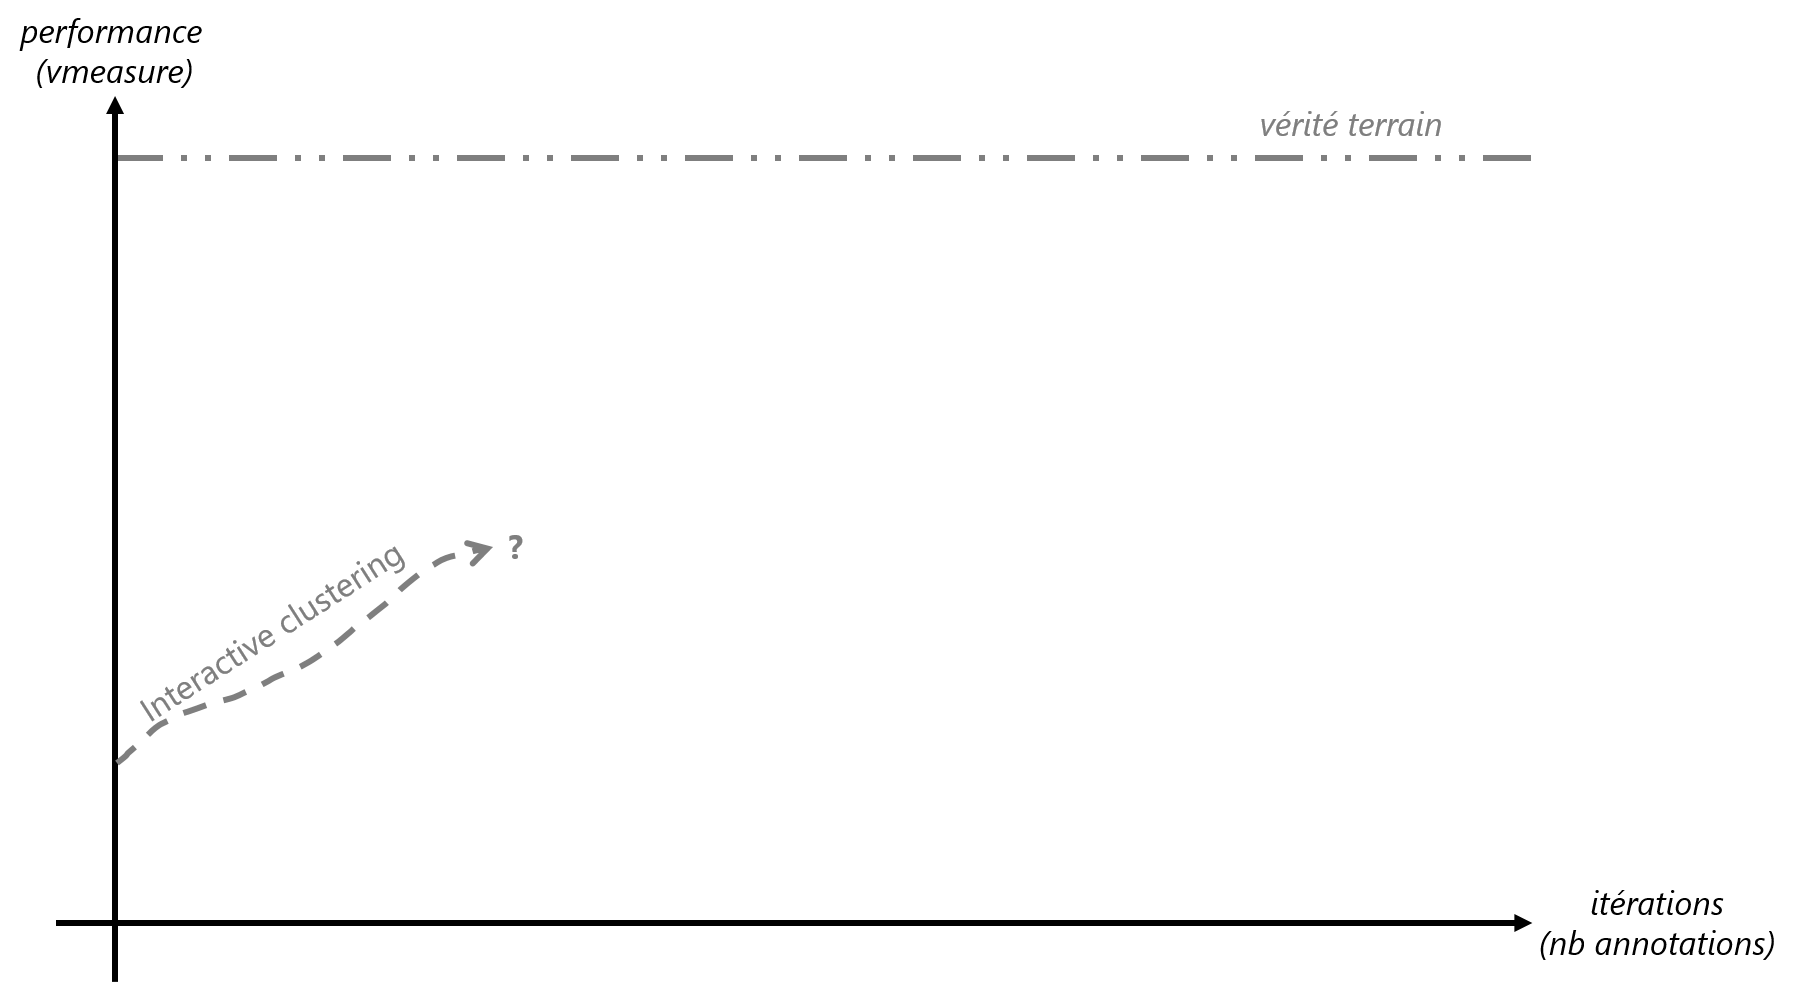
\includegraphics[width=0.8\textwidth]{figures/hypotheses-00-default}
		\caption{Illustration des études réalisées sur le \textit{clustering} interactif (\textit{étape 0/6}) en schématisant l'évolution de la performance (\textit{accord avec la vérité terrain calculé en v-measure}) d'une base d'apprentissage en cours de construction en fonction du nombre d'itérations de la méthode (\textit{nombre d'annotations par un expert métier}).}
		\label{figure:HYPOTHESE-00-DEFAULT}
	\end{figure}
	
	% PRÉAMBULE TECHNIQUE : CPU + scrips + datasets.
	Pour ces études, l'exécution des différentes expériences a été réalisée sur des CPU \textit{Intel(R) Xeon(R) CPU E5-2660 v4 \@ 2.00GHz} et parallélisé avec la librairie Python \textit{multiprocessing} (un worker par CPU).
	Les scripts d'exécution et d'analyse de ces expériences, rédigés au sein de notebooks Python et/ou R, sont disponibles dans~\cite{schild:cognitivefactory-interactive-clustering-comparative-study:2021}\todo{footnote documentation}.
	Enfin, les jeux de données utilisés pour ces études sont détaillés en Annexe~\ref{annex:C-ANNEXE-DATASET}.
	
	
	% TABLE DES MATIÈRES DU CHAPITRE
    \minitoc

    %%%%%--------------------------------------------------------------------
    %%%%% Section 4.1: Hypothèse d'efficacité.
    %%%%%--------------------------------------------------------------------
    \section{Hypothèse d'efficacité : « \textit{est-ce que la méthode fonctionne ?} »}
	\label{section:4.1-HYPOTHESE-EFFICACITE}
	
		%%% Formulation des hypothèses:
		Nous aimerions vérifier l'hypothèse suivante :

		\begin{tcolorbox}[
			title=\textbf{Hypothèse d'efficacité},
			colback=gray!20,
			colframe=gray!50!black!75,
			width=\linewidth
		]
			% « Une méthodologie d'annotation basée sur le \textit{clustering} interactif \textbf{peut converger} vers une vérité terrain préalablement établie (cf. figure~\ref{figure:HYPOTHESE-EFFICACITE}. »
			« \textbf{
				Une méthodologie d'annotation basée sur le \textit{clustering} interactif permet d'obtenir une base d'apprentissage pour un assistant conversationnel qui respecte la vision donnée par l'expert métier au cours de l'annotation.
			} » \\
			
			Afin de vérifier cette hypothèse, nous mettrons en place une expérience de ré-annotation d'une base d'apprentissage (qui servira ici de vérité terrain) à l'aide de notre méthode, en simulant l'annotation d'un expert, et nous critiquerons l'évolution de la nouvelle base d'apprentissage obtenue et sa similitude avec la base d'apprentissage initiale.
			
			La figure~\ref{figure:4.1-HYPOTHESE-EFFICACITE} illustre l'hypothèse et l'espoir de convergence d'une base d'apprentissage en cours de construction vers sa vérité terrain.
			%
			\begin{figure}[H]
				\centering
				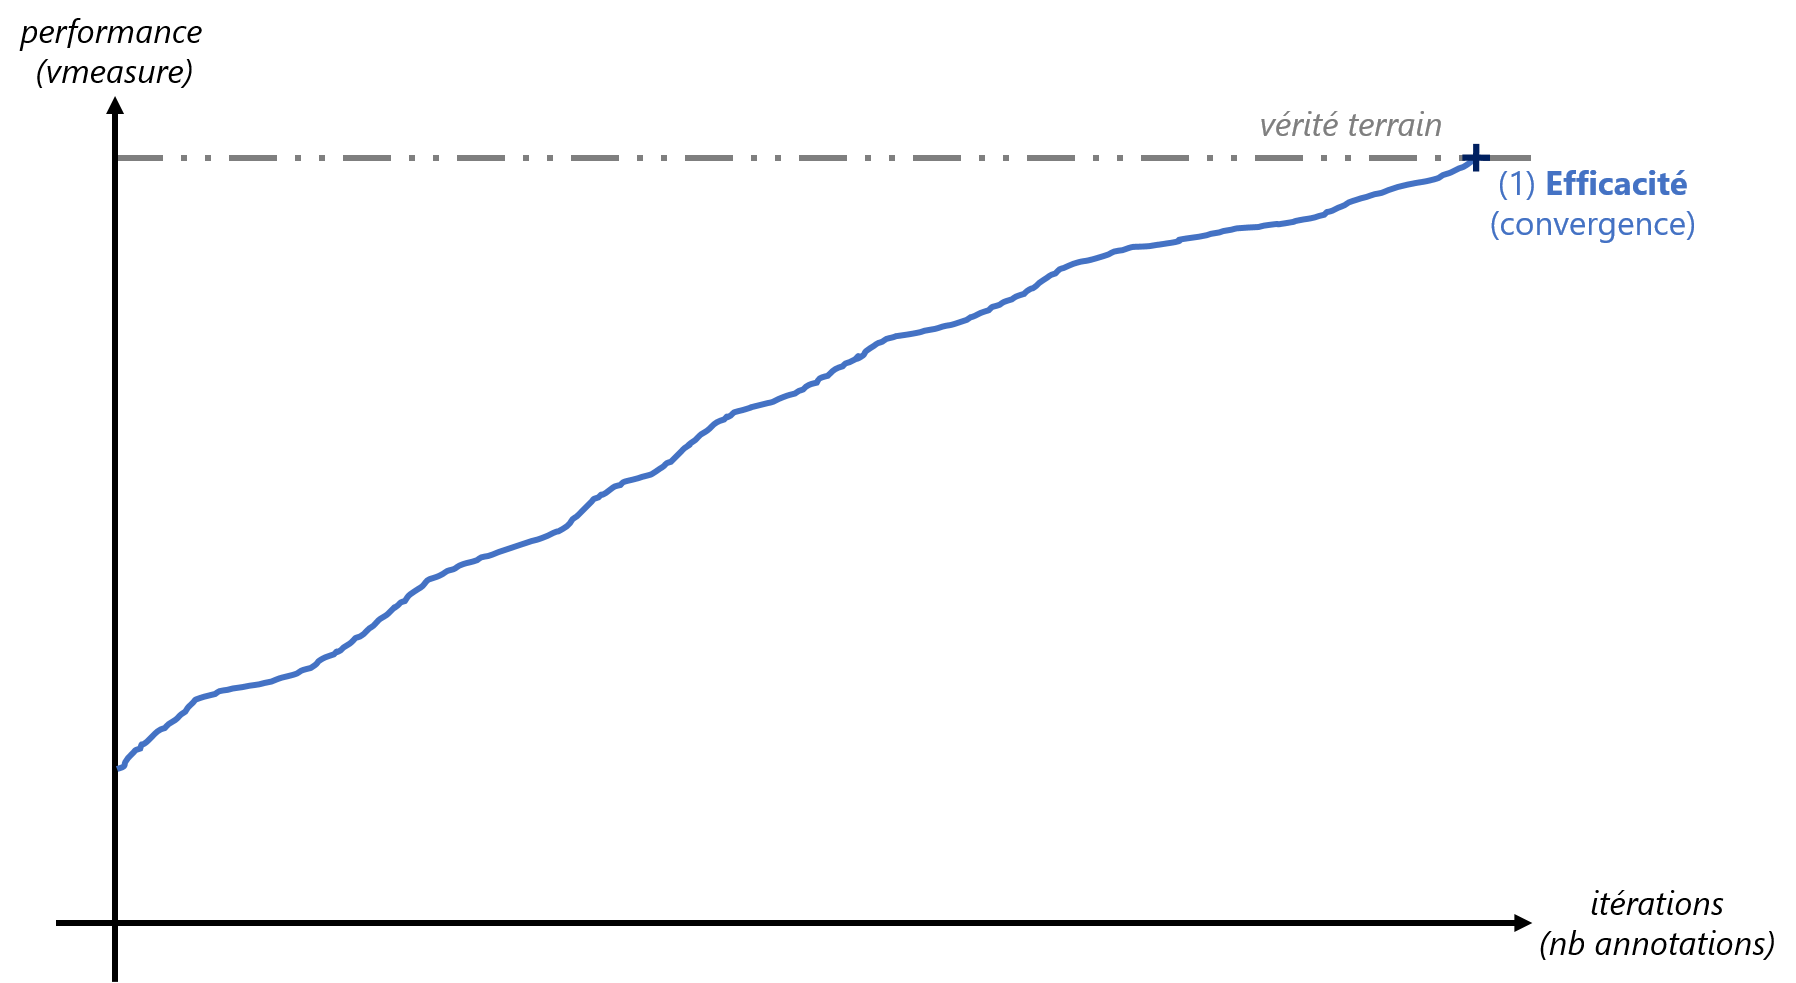
\includegraphics[width=0.8\textwidth]{figures/hypotheses-01-efficacite}
				\caption{Illustration des études réalisées sur le \textit{clustering} interactif (\textit{étape 1/6}) en schématisant l'évolution de la performance (\textit{accord avec la vérité terrain calculé en v-measure}) d'une base d'apprentissage en cours de construction en fonction du nombre d'itérations de la méthode (\textit{nombre d'annotations par un expert métier}).}
				\label{figure:4.1-HYPOTHESE-EFFICACITE}
			\end{figure}

		\end{tcolorbox}
		
		%%%
		%%% Subsection 4.1.1: Étude de convergence
		%%%
		\subsection{Étude de convergence vers une vérité terrain pré-établie}
		\label{subsection:4.1.1-ETUDE-CONVERGENCE}
				
			% Référence articles.
			Cette étude a été l'objet d'une présentation à la conférence \texttt{EGC (Extraction et Gestion des Connaissances)}~\citep{schild:conception-interactive-clustering:2021}, et d'une extension dans le journal \texttt{IJDWM (International Journal of Data Warehousing and Mining)}~\citep{schild:extension-interactive-clustering:2022}.
	
			%%% Protocole expérimental.
			\subsubsection{Protocole expérimental : simuler l'annotation d'une base d'apprentissage}
			
				% Objectif de l'expérience.
				Nous voulons vérifier qu'une méthodologie d'annotation basée sur notre implémentation du \textit{clustering} interactif permet de créer une base d'apprentissage pour un assistant conversationnel.
				Pour cela, nous prenons une base d'apprentissage employée pour entraîner un modèle de classification de textes\todo{référence, lien vers ANNEXE}, et nous utilisons ce jeu de données comme vérité terrain.
				L'objectif de cette expérience est de simuler la création de cette base d'apprentissage et de nous assurer que le résultat obtenu correspond à la vérité terrain.
				% Axiome.
				Dans le cadre de cette étude, nous supposons que l'expert métier connaît parfaitement le domaine traité dans ce jeu de données, et qu'il est capable de caractériser sans ambiguïté la similitude entre deux données issues de cet ensemble.\todo{Ajouter format spécial pour cette note ?}
				
				% Détails de l'expérience.
				Lors de cette expérience, chaque tentative de la méthode commencera sur la version non labellisée de la vérité terrain à disposition, sans aucune contrainte connue à l'avance.
				Au fur et à mesure des itération de la méthode, nous simulerons l'annotation de l'expert métier en comparant les labels de la vérité terrain : ainsi, deux données ont une contrainte \texttt{MUST-LINK} si elles ont le même label, et une contrainte \texttt{CANNOT-LINK} sinon. Cela traduit le prérequis d'avoir un annotateur qui soit capable de critiquer la ressemblance entre deux données de son domaine d'expertise.
				Une tentative de l'application de notre méthode s'arrête lorsque toutes les contraintes possibles entre les données ont été annotés par l'expert.

				% Description implémentation de l'interactive clustering.
				Pour cette étude, nous essayons une tentative pour chaque combinaison de paramètre de notre implémentation du clustering interactif (cf. section~\ref{section:3.3-DESCRIPTION-IMPLEMENTATION}). Cela comprend les tâches et leurs paramètres respectifs suivants :
				%
				\begin{enumerate}
					\item le \textbf{prétraitement} des données, avec les quatre niveaux suivants : \texttt{prep.no}, \texttt{prep.simple}, \texttt{prep.lemma} et \texttt{prep.filter} ;
					\item la \textbf{vectorisation} des données, avec les deux niveaux suivants : \texttt{vect.tfidf} et \texttt{SpaCy (vect.frcorenewsmd)} ;
					\item le \textbf{clustering sous contraintes} des données, avec les six niveaux suivants : \texttt{clust.kmeans.cop}, \texttt{clust.hier.sing}, \texttt{clust.hier.comp}, \texttt{clust.hier.avg}, \texttt{clust.hier.ward} et \texttt{clust.spec}. Le choix du nombre de clusters n'est pas étudié ici, et ce nombre est fixé au nombre de classes présentes dans la vérité terrain ;\todo{ Tester C-DBScan ? }
					\item l'\textbf{échantillonnage} des contraintes à annoter, avec les quatre niveaux suivants : \texttt{samp.random.full}, \texttt{samp.random.same}, \texttt{samp.farhtest.same} et \texttt{samp.closest.diff}. La choix de la taille d'échantillon n'est pas étudié ici, et cette taille est arbitrairement fixé à \texttt{50}.
				\end{enumerate}
				
				Il y a donc 192 combinaisons testées, et chaque tentative est répétée 5 fois pour contrer les aléas statistiques de certains algorithmes.
				Pour plus de détails sur ces algorithmes, référez-vous à la section~\ref{section:3.3-DESCRIPTION-IMPLEMENTATION} pour avoir accès à leur description, à leurs paramètres et aux choix d'implémentation.
				
				% Description de l'évaluation.
				Pour évaluer l'équivalence entre la vérité terrain et notre segmentation des données obtenue au cours de la méthode, nous nous intéresserons à l'évolution de la \texttt{v-measure} entre ces deux jeu de données.
				Si le score du calcul de la \texttt{v-measure} est de \texttt{100\%}, cela signifierait que le clustering final et la vérité terrain propose une segmentation identique des données, donc que la vérité terrain a pu être retrouvée, et donc qu'il est possible d'obtenir une base d'apprentissage pour un assistant conversationnel à l'aide d'une méthodologie d'annotation basée sur le \textit{clustering} interactif.
				
				% Seuils d'évaluation.
				Afin d'affiner notre évaluation, nous porterons aussi attention aux seuils d'annotations suivants :
				%
				\begin{enumerate}
					\item le \textbf{\textit{clustering} initial}, correspondant à la segmentation des données sans contraintes, ne bénéficiant d'aucune connaissance métier ;
					\item le cas d'une \textbf{annotation suffisante}, correspondant au nombre d'itérations nécessaires à la méthode pour avoir 100\% de \texttt{v-measure} entre le résultat obtenu et la vérité terrain, c'est-à-dire avoir suffisamment de contraintes annotées par l'expert métier pour retrouver la vérité terrain ;
					\item le cas d'une \textbf{annotation exhaustive}, correspondant au nombre d'itérations nécessaires à la méthode pour parcourir toutes les contraintes possibles sur les données, et ainsi retranscrire exhaustivement la vision de l'expert métier.
				\end{enumerate}
				
				% Pseudo-code.
				Pour résumer ce protocole expérimental, vous pouvez vous référez au pseudo-code décrit dans Alg.~\ref{algorithm:4.1.1-ETUDE-CONVERGENCE-PROTOCOLE}.
				%
				\begin{algorithm}
					\begin{algorithmic}[1]
						\Require jeu de données annoté (vérité terrain)
						\ForAll{arrangement d'algorithmes et de paramètres à tester}
							\State \textbf{initialisation}: récupérer les données de la vérité terrain sans leur label, créer une liste vide de contraintes
							\State \textbf{prétraitement}: supprimer le bruit dans les données
							\State \textbf{vectorisation}: transformer les données en vecteurs
							\State \textbf{clustering initial}: regrouper les données par similarité
							\State \textbf{évaluation}: estimer l'équivalence entre le clustering obtenu et la vérité terrain
							\Repeat
								\State \textbf{échantillonnage}: sélectionner de nouvelles contraintes à annoter
								\State \textbf{simulation d'annotation}: ajouter des contraintes grâce à la comparaison des labels de la vérité terrain
								\State \textbf{clustering}: regrouper les données par similarité avec les contraintes
								\State \textbf{évaluation}: estimer l'équivalence entre le clustering obtenu et la vérité terrain
							\Until{annotation de toutes les contraintes possibles}
							\State \textbf{évaluation finale}: espérer avoir un score d'équivalence de 100\% entre le clustering obtenu et la vérité terrain
						\EndFor
						\Ensure arrangements d'algorithmes et de paramètres ayant un score d'équivalence de 100\%
					\end{algorithmic}
					\caption{Description en pseudo-code du protocole expérimental de l'étude de convergence du \textit{clustering} interactif vers une vérité terrain pré-établie.}
					\label{algorithm:4.1.1-ETUDE-CONVERGENCE-PROTOCOLE}
				\end{algorithm}
				
				% Référence scripts.
				Les scripts de l'expérience (\textit{notebooks} Python) sont disponibles dans un dossier dédié de~\cite{schild:cognitivefactory-interactive-clustering-comparative-study:2021}.

			%%% Résultats.
			\subsubsection{Résultats obtenus}
				
				% Toutes les tentatives convergent.
				Toutes les 960 tentatives (192 combinaisons de paramètres, 5 tentatives pour chaque combinaison) ont convergé vers la vérité terrain (i.e. on atteint une \texttt{v-measure} de 100\%).
				% Graphe d'évolution de la v-measure moyenne, min et max.
				La figure~\ref{figure:4.1.1-ETUDE-CONVERGENCE-EVOLUTION} représente l'évolution moyenne de la \texttt{v-measure} du clustering en fonction du nombre d'itération de la méthode. Les tentatives les plus rapides et les plus lentes y sont aussi représentées.
				%
				\begin{figure}[H]
					\centering
					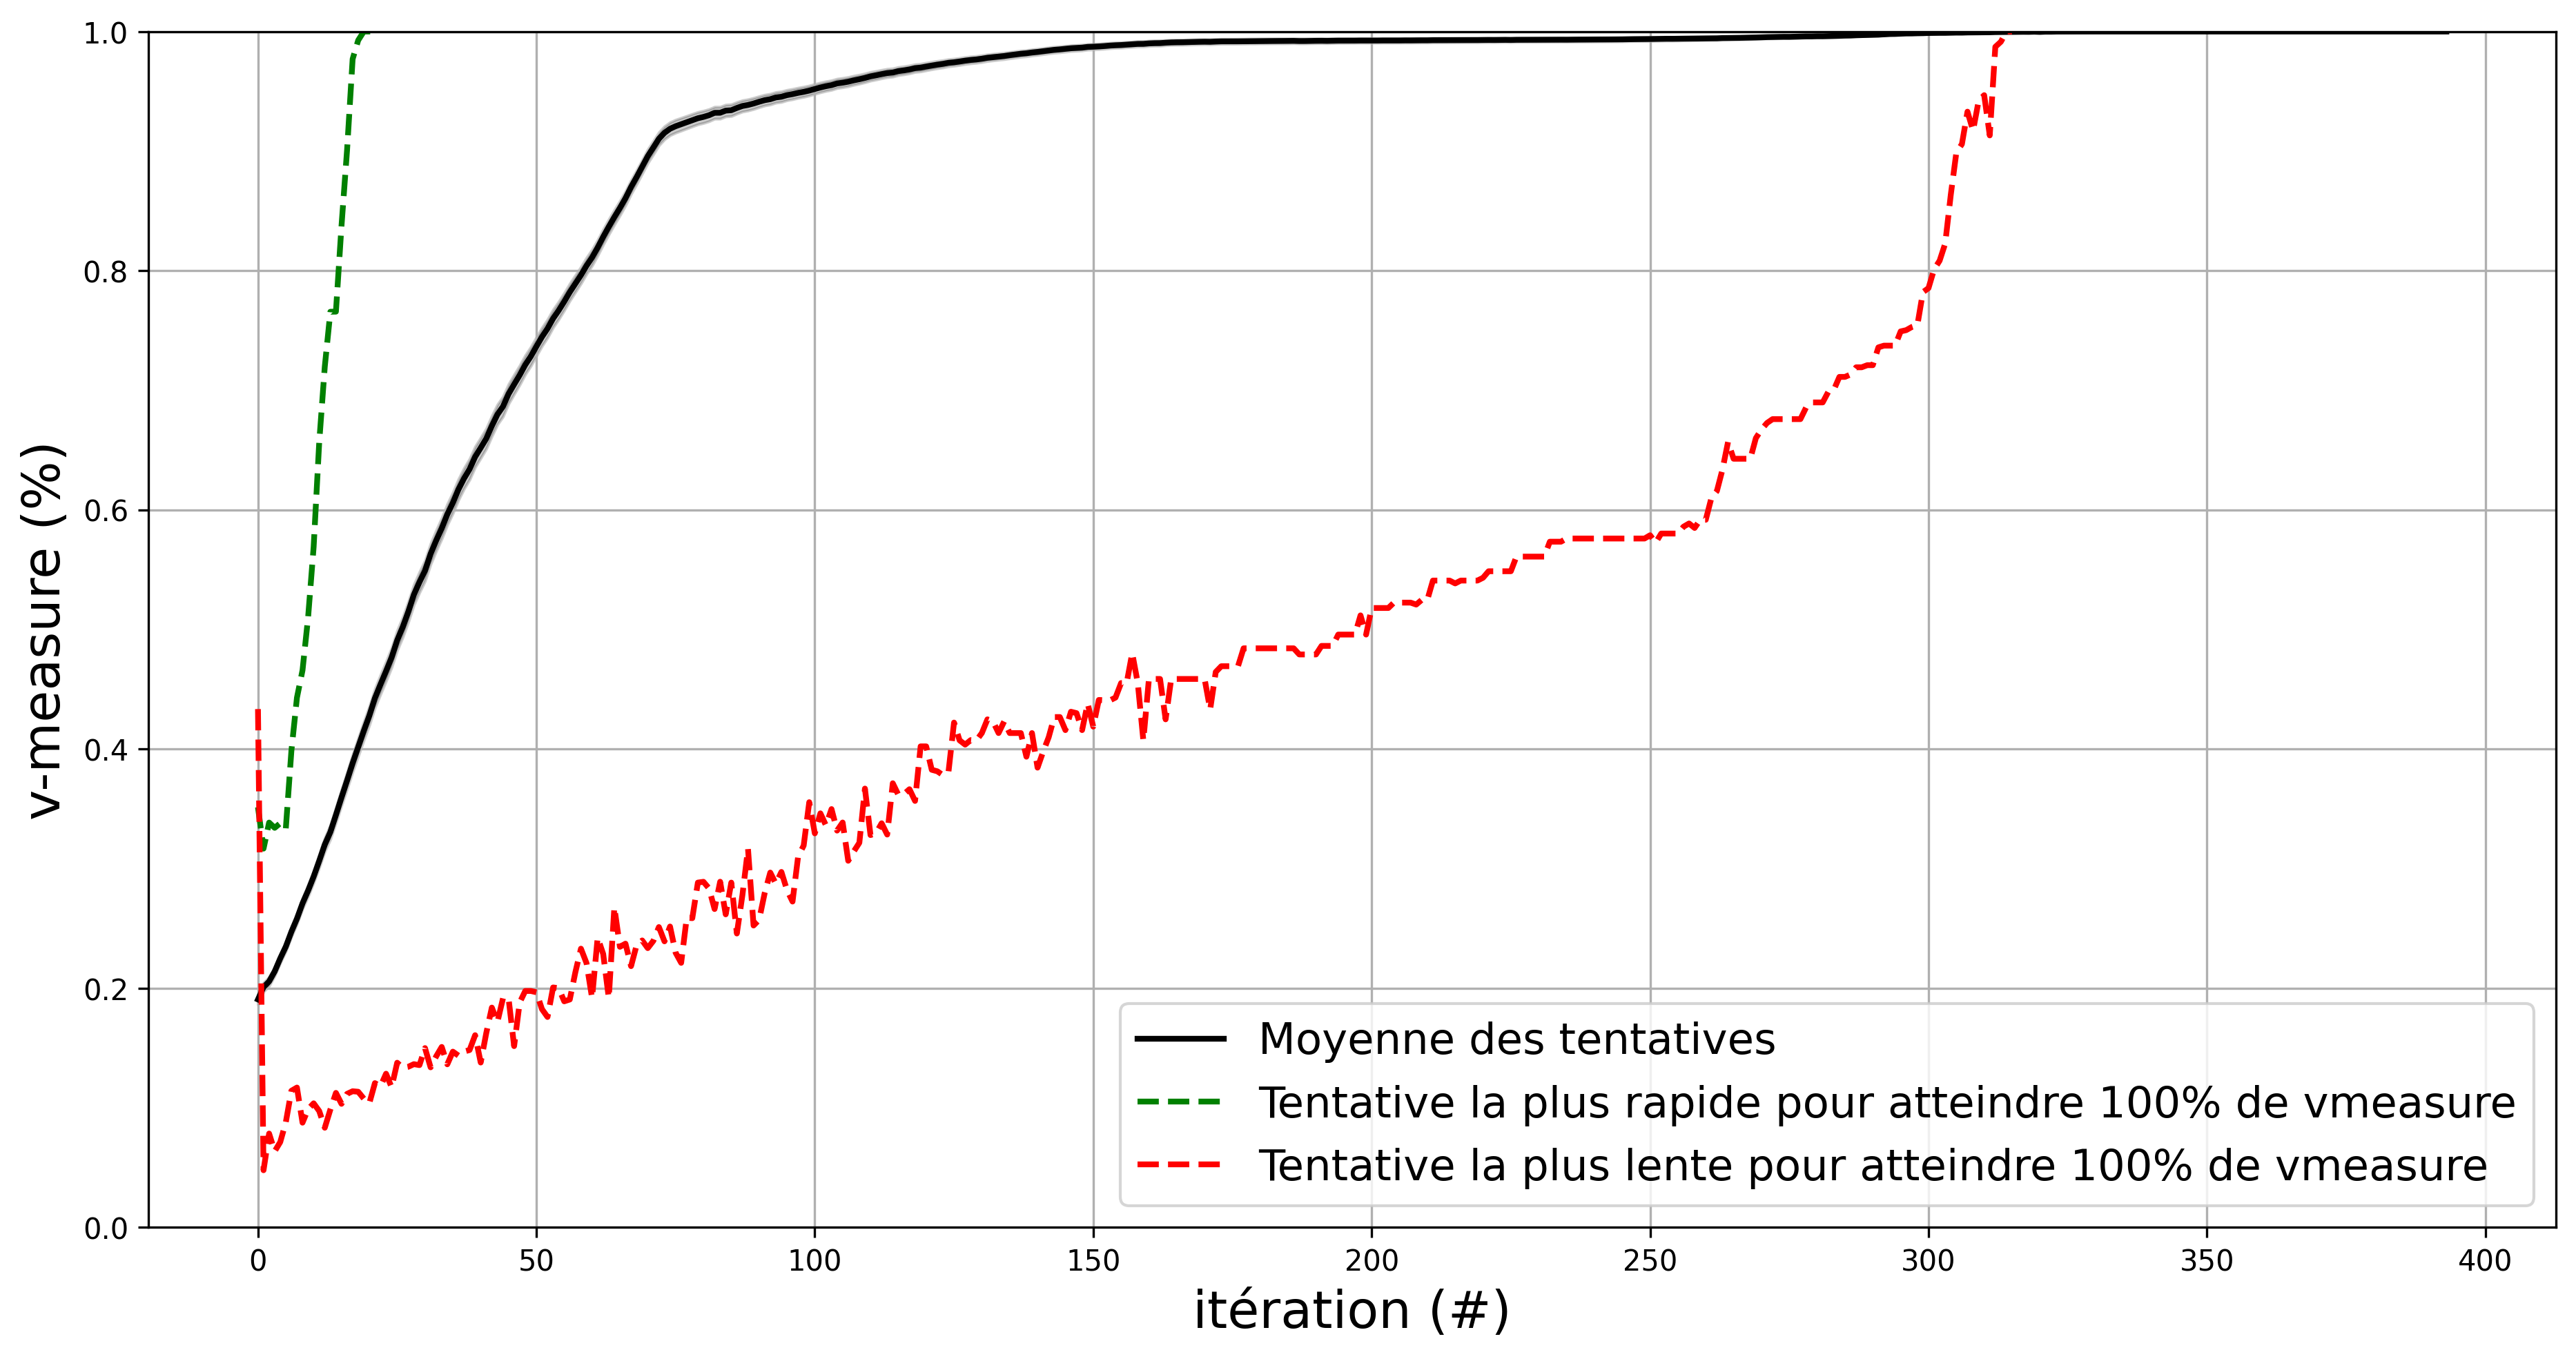
\includegraphics[width=0.8\textwidth]{figures/etude-convergence-evolution-moyenne-0par-iteration}
					\caption{Évolution de la moyenne de la \texttt{v-measure} entre un résultat obtenu et la vérité terrain en fonction du nombre d'itération de la méthode de \textit{clustering} interactif, moyenne réalisée itération par itération sur l'ensemble des tentatives.
					Représentation des tentatives ayant été les plus rapides (\textit{un prétraitement \texttt{prep.simple}, une vectorisation \texttt{vect.tfidf}, un clustering \texttt{clust.hier.comp} ou \texttt{clust.hier.ward}, et un échantillonnage \texttt{samp.closest.diff}}) et les plus lentes (\textit{un prétraitement \texttt{prep.no}, une vectorisation \texttt{vect.tfidf}, un clustering \texttt{clust.spec}, et un échantillonnage de contraintes \texttt{samp.farthest.same}}) pour atteindre 100\% de \texttt{v-measure}.}
					\label{figure:4.1.1-ETUDE-CONVERGENCE-EVOLUTION}
				\end{figure}
				
				
				% Analyse du clustering initial.
				Lors du \textbf{\textit{clustering} initial}, on remarque que la \texttt{v-measure} entre le clustering (sans contraintes) et la vérité terrain atteint une moyenne de \texttt{19.05}\% (min: \texttt{03.42}\%, max: \texttt{47.75}\%, écart-type: \texttt{13.38}\%) ;
				
				% Analyse d'une annotation suffisante.
				Pour obtenir une \textbf{annotation suffisante} (\textit{atteindre une \texttt{v-measure} de 100\%}), la moyenne des itérations est de \texttt{76.29} (min: \texttt{19}, max: \texttt{328}, écart-type: \texttt{46.44}), soit une moyenne de \texttt{3 801.19} annotations (min: \texttt{950}, max: \texttt{16 400}, écart-type: \texttt{2 314.91}).
				La figure~\ref{figure:4.1.1-ETUDE-CONVERGENCE-HISTOGRAMME-ANNOTATION-SUFFISANTE} représente la répartition de ces itérations au cours des différentes tentatives.
				On peut noter les deux cas intéressants suivant :
				%
				\begin{itemize}
					\item[\(\bullet\)] Les tentatives les plus rapides furent avec un prétraitement \texttt{prep.simple}, une vectorisation \texttt{vect.tfidf}, un clustering \texttt{clust.hier.comp} ou \texttt{clust.hier.ward}, et un échantillonnage \texttt{samp.closest.diff}. Ces tentatives ont requis \texttt{19} itérations, soit \texttt{950} annotations, dont \texttt{638} (respectivement \texttt{641}) contraintes \texttt{MUST-LINK}.
					\item[\(\bullet\)] Les tentatives les plus lentes furent avec prétraitement \texttt{prep.no}, une vectorisation \texttt{vect.tfidf}, un clustering \texttt{clust.spec}, et un échantillonnage de contraintes \texttt{samp.farthest.same}. Ces tentatives ont requis \texttt{394} itérations, soit \texttt{16 400} annotations, dont \texttt{1 309} contraintes \texttt{MUST-LINK}.
				\end{itemize}
				%
				\begin{figure}[H]
					\centering
					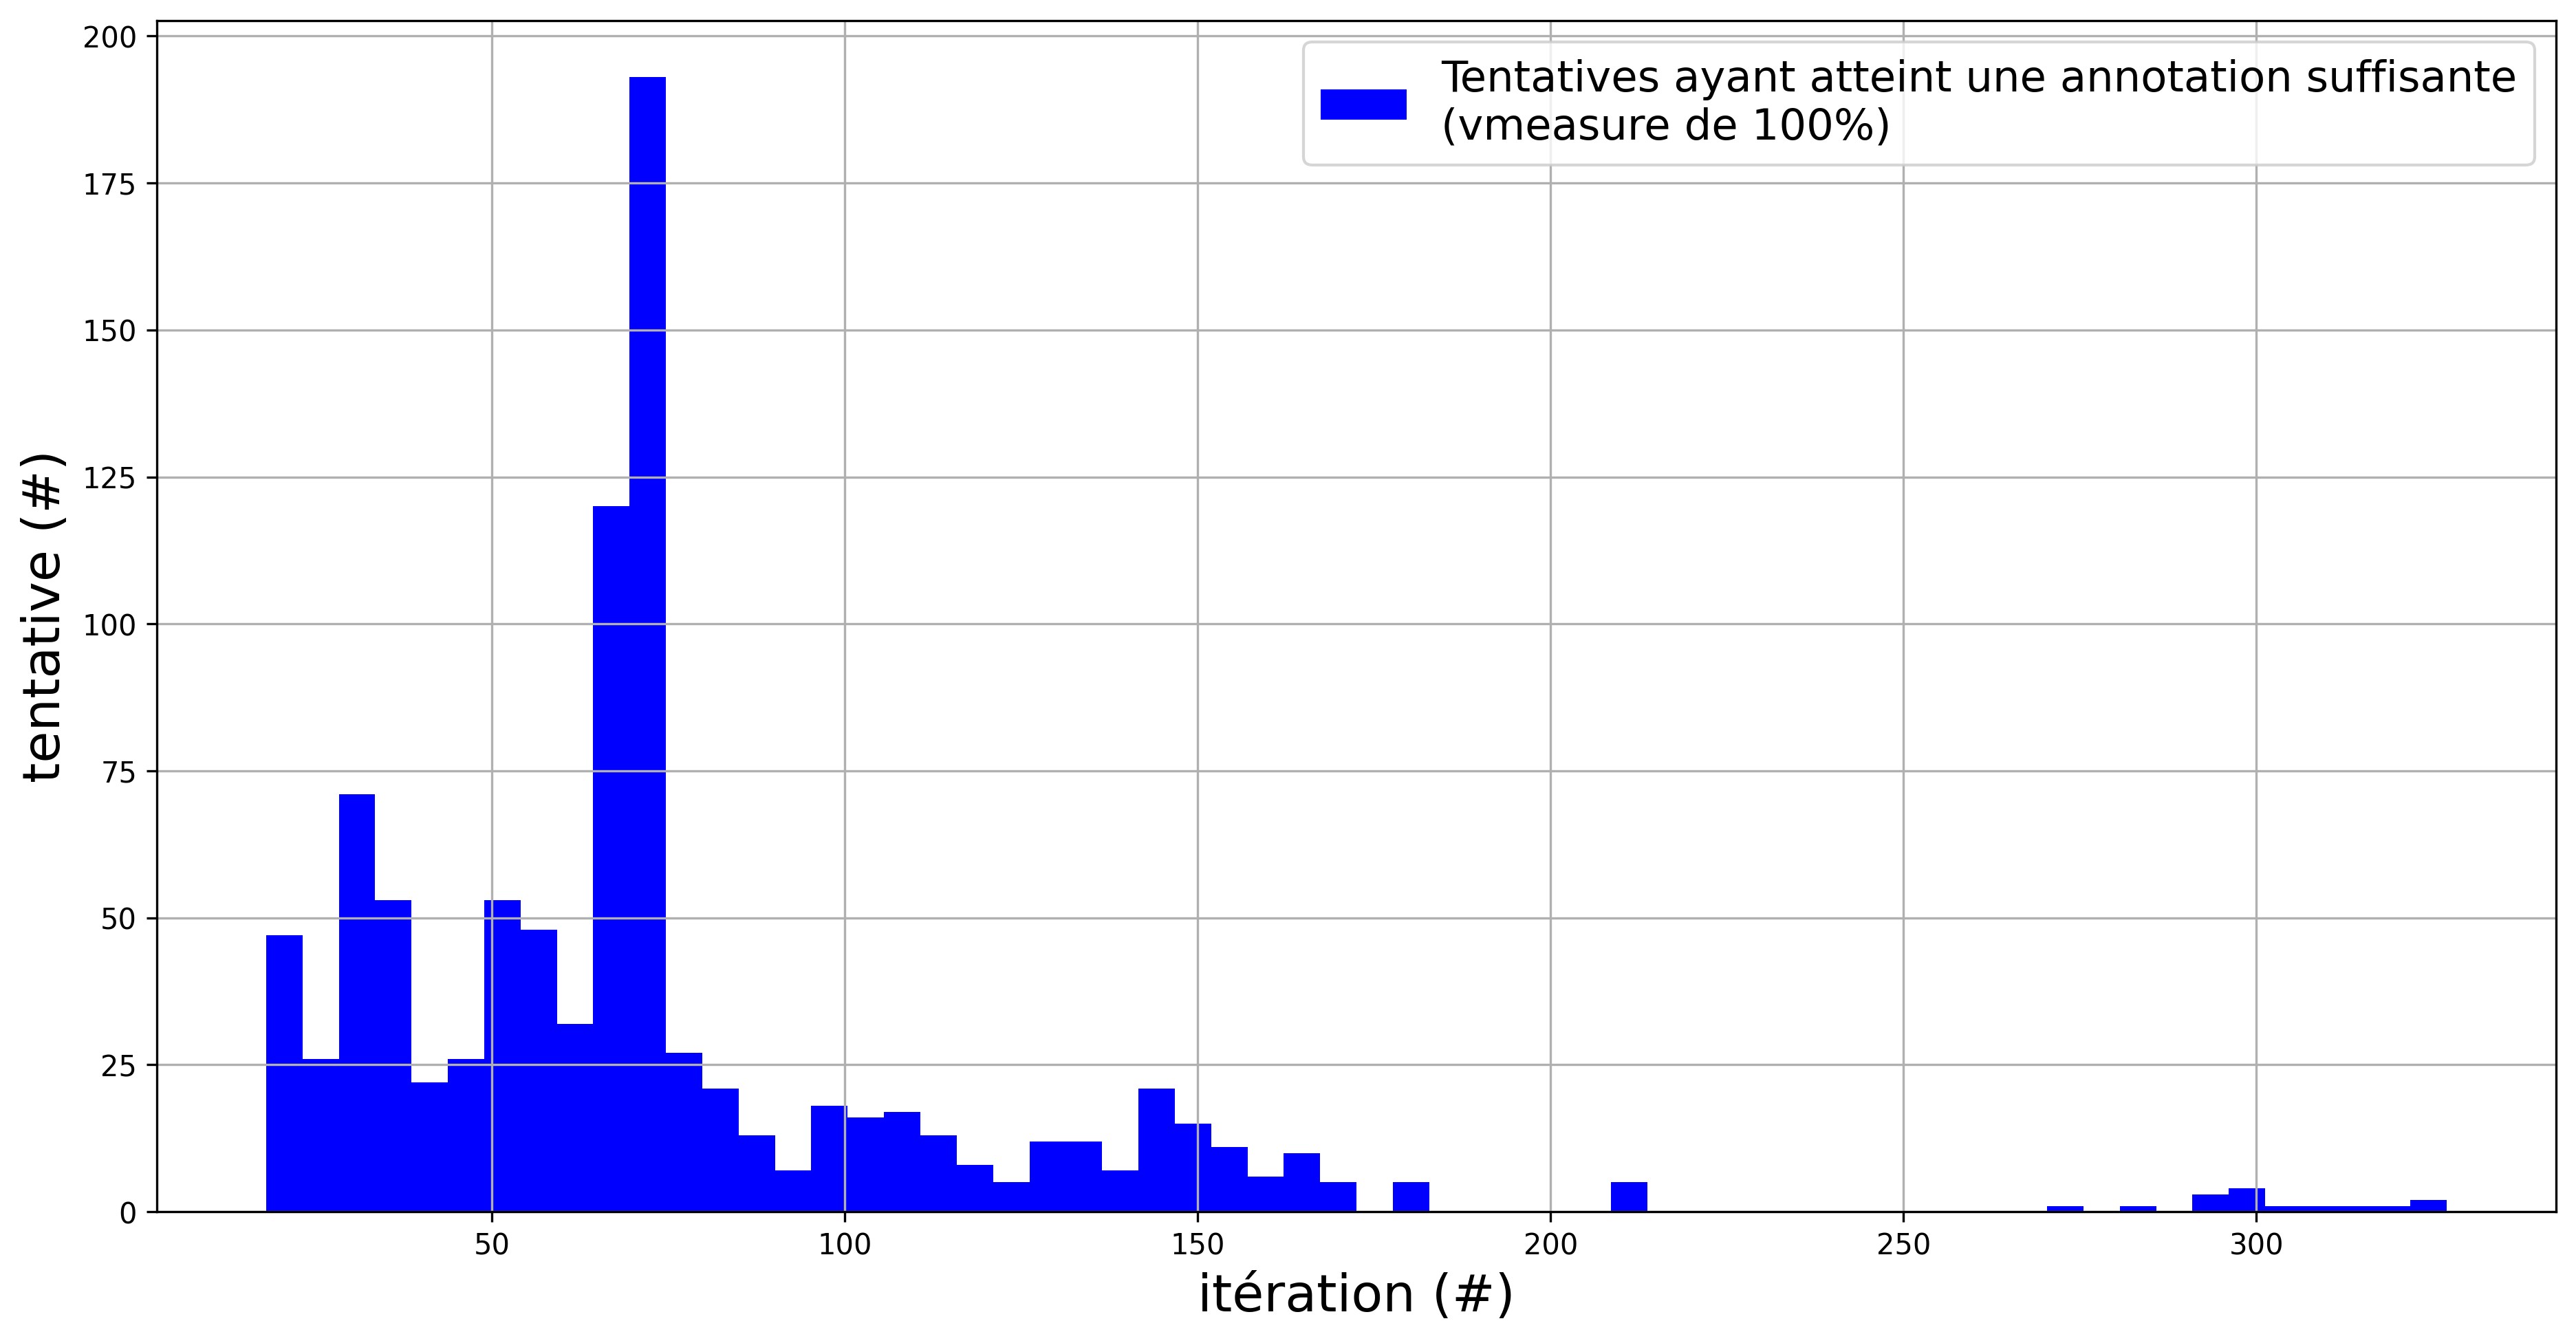
\includegraphics[width=0.8\textwidth]{figures/etude-convergence-histogramme-annotation-suffisante}
					\caption{Répartition des tentatives en fonction de l'itération de la méthode à laquelle elles atteignent le seuil d'une annotation suffisante, c'est-à-dire l'itération à laquelle elles parviennent à 100\% de \texttt{v-measure} entre un résultat obtenu et la vérité terrain. La moyenne est située à \texttt{76.29} itérations, et l'histogramme est réduit à 60 pics pour simplifier l'affichage.}
					\label{figure:4.1.1-ETUDE-CONVERGENCE-HISTOGRAMME-ANNOTATION-SUFFISANTE}
				\end{figure}
				
				
				% Analyse d'une annotation exhaustive.
				Enfin, pour avoir une \textbf{annotation exhaustive} (\textit{annoter toutes les contraintes possibles}), la moyenne des itérations est de \texttt{88.98} (min: \texttt{20}, max: \texttt{394}, écart-type: \texttt{68.21}), soit une moyenne de \texttt{4 431.34} annotations (min: \texttt{1 000}, max: \texttt{19 656}, écart-type: \texttt{3 405.16}).
				La figure~\ref{figure:4.1.1-ETUDE-CONVERGENCE-HISTOGRAMME-ANNOTATION-EXHAUSTIVE} représente la répartition de ces itérations au cours des différentes tentatives.
				On peut noter les deux cas intéressants suivant :
				%
				\begin{itemize}
					\item[\(\bullet\)] Les tentatives les plus rapides furent avec un prétraitement \texttt{prep.no} ou \texttt{prep.lemma}, une vectorisation \texttt{vect.tfidf}, un clustering \texttt{clust.hier.comp} ou \texttt{clust.hier.wars}, et un échantillonnage de contraintes \texttt{samp.closest.diff}. Ces tentatives ont requis \texttt{20} itérations, soit \texttt{1 000} annotations, dont \texttt{653} (respectivement \texttt{668}) contraintes \texttt{MUST-LINK}.
					\item[\(\bullet\)] Les tentatives les plus lentes furent avec un prétraitement \texttt{prep.simple}, une vectorisation \texttt{vect.frcorenewsmd}, un clustering \texttt{clust.hier.sing}, et un échantillonnage \texttt{samp.closest.diff}. Ces tentatives ont requis \texttt{394} itérations, soit \texttt{19 656} annotations, dont \texttt{682} contraintes \texttt{MUST-LINK}.
				\end{itemize}
				%
				\begin{figure}[H]
					\centering
					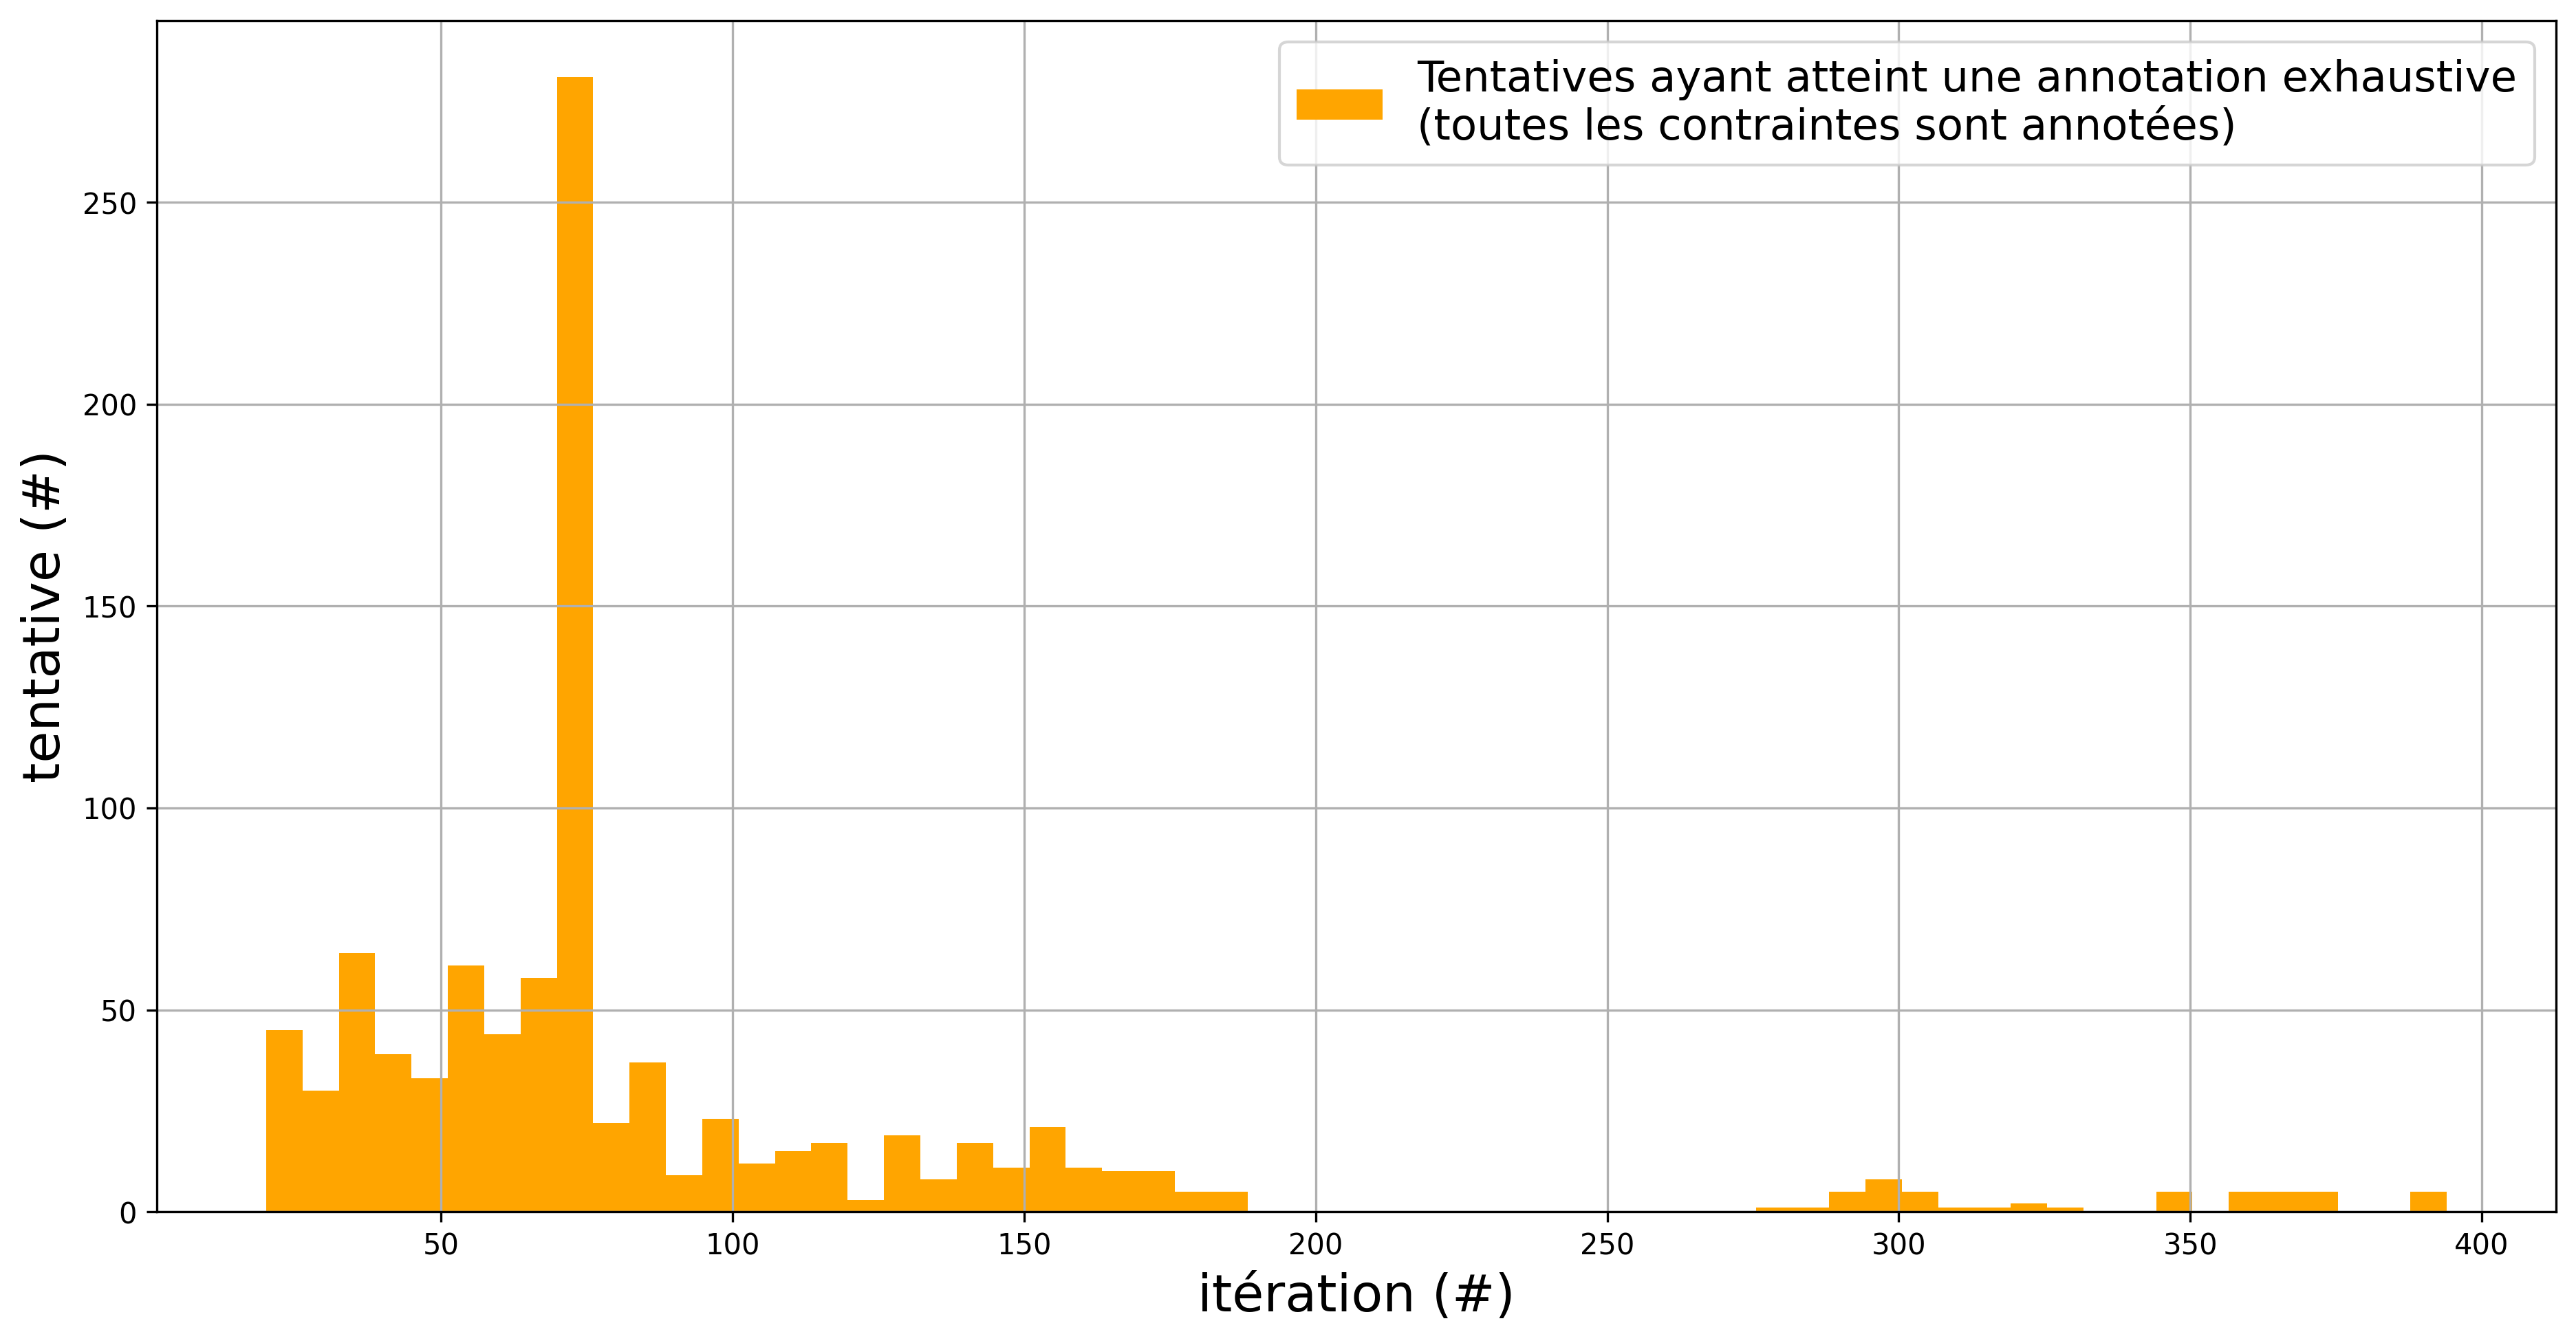
\includegraphics[width=0.8\textwidth]{figures/etude-convergence-histogramme-annotation-exhaustive}
					\caption{Répartition des tentatives en fonction de l'itération de la méthode à laquelle elles atteignent le seuil d'une annotation exhaustive, c'est-à-dire l'itération à laquelle toutes les contraintes possibles entre les données ont été annotées. La moyenne est située à \texttt{88.98} itérations, et l'histogramme est réduit à 60 pics pour simplifier l'affichage.}
					\label{figure:4.1.1-ETUDE-CONVERGENCE-HISTOGRAMME-ANNOTATION-EXHAUSTIVE}
				\end{figure}

			%%% Discussion
			\subsubsection{Discussion}
				
				%%% Principale conclusion : il y a convergence !
				La première et principale conclusion de cette étude concerne la preuve que la méthode est fonctionnelle.
				En effet, les différentes simulations ont bien convergé vers la vérité terrain, montrant qu'il est possible pour un expert métier de créer une base d'apprentissage à l'aide d'une méthodologie d'annotation basée sur le \textit{clustering} interactif. \\
				
				
				%%% Avantages.
				Cette découverte permet de confirmer plusieurs espoirs porter sur la méthode. 
				
				% Avantage 1 : Émergence d'une modélisation sur la base des contraintes
				Tout d'abord, la vérité terrain a été retrouvée sans formaliser concrètement la structure de données.
				Là où une annotation par label aurait requis au préalable une définition des catégories de données possibles, la méthodologie employant le \textit{clustering} interactif a permis de faire émerger naturelle cette structure de données.
				Cette émergence provient directement des contraintes annotées par l'expert métier, traduisant par elles ses connaissances à l'aide d'instructions simples : les données sont-elles ou non similaires ?
				
				% Avantage 2 : annotations plus simples et plu concrètes
				De plus, ces contraintes ont été l'objet d'une annotation guidée par les besoins de la machine afin de s'améliorer d'itération en itération (voir la croissance de la \texttt{v-measure} sur la figure~\ref{figure:4.1.1-ETUDE-CONVERGENCE-EVOLUTION}).
				A chaque itération, l'expert métier peut ainsi corriger concrètement la base d'apprentissage, soit étendant les clusters en cours de construction (pics de croissance sur la courbe), soit en remaniant les clusters mal formés pour imposer sa vision (légères décroissances sur la courbe). \\

				
				%%% Les limites.
				Néanmoins, différentes pistes sont encore à explorer pour rendre le \textit{clustering} interactif pleinement opérationnel.
				
				% Limite 1 : Nombre d'annotations ==> besoin d'optimisation.
				D'une part, nous échangeons le besoin de définir une structure de données contre la nécessité d'annoter un grand nombre de contraintes afin de converger vers la vérité terrain : pour \texttt{500} points de données, il faudrait une moyenne de \texttt{76.29} itérations, soit \texttt{3 801.19} annotations, ce qui correspond à près de \texttt{8} fois plus de contraintes que de données.
				Bien que l'annotation binaire demande a priori une charge mentale plus faible à un annotateur, un tel volume représente une grande quantité de travail, peut effrayer les experts métiers, mais peut aussi ne pas être viable pour des jeux de données de plus grandes tailles.
				Cependant, les résultats obtenus montrent une forte dispersion du nombre d'itérations nécessaire (écart-type de \texttt{46.44}).
				On peut donc espérer trouver un paramétrage optimal de la méthode permettant de diminuer significativement le nombre de contraintes requis et obtenir ainsi une base d'apprentissage exploitable avec une charge d'annotation maîtrisée.
				Cet aspect fait l'objet de l'étude décrite dans la section~\ref{section:4.2-HYPOTHESE-EFFICIENCE} (hypothèse d'efficience).\todo{footnote ?}
				
				% Limite 2 : Expert métier parfait ==> simuler les erreurs.
				D'autre part, nous avons supposé dans cette étude que l'annotateur est un expert métier connaissant parfaitement le domaine traité.
				Cette hypothèse forte n'est a priori pas valable en situation réelle : En effet, des erreurs d'annotations peuvent intervenir (ambiguïtés sur les données, méconnaissance du domaine, erreurs d'inattention, différence d'opinions entre annotateurs, ...), ce qui peut entraîner des divergences ou des incohérences dans la base d'apprentissage en cours de construction.
				Il semble donc nécessaire d'étudier les impacts de ces incohérences, ainsi que de proposer une méthode pour les identifier et les corriger.
				Cet aspect sera traité à la fin de ce chapitre lors de la section~\ref{section:4.6-HYPOTHESE-ROBUSTESSE} (hypothèse de robustesse).
	

    %%%%%--------------------------------------------------------------------
    %%%%% Section 4.2: Hypothèse d'efficience.
    %%%%%--------------------------------------------------------------------
    \section{Hypothèse d'efficience : « \textit{est-ce que l'implémentation est optimale ?} »}
	\label{section:4.2-HYPOTHESE-EFFICIENCE}
	
		%%% Formulation des hypothèses:
		Nous aimerions vérifier l'hypothèse suivante :
		\todo{à compléter}

		\begin{tcolorbox}[
			title=\textbf{Hypothèse d'efficience},
			colback=gray!20,
			colframe=gray!50!black!75,
			width=\linewidth
		]

			% « La vitesse de convergence du \textit{clustering} interactif \textbf{peut être optimisée} en ajustant différents paramètres. Nous étudierons en particulier l'influence du prétraitement des données, de la vectorisation des données, de l'échantillonnage des contraintes à annoter et du \textit{clustering} sous contraintes (cf. figure~\ref{figure:HYPOTHESE-EFFICIENCE}. »
			« \textbf{
				La vitesse de convergence du \textit{clustering} interactif peut être optimisée en ajustant différents paramètres. Nous étudierons en particulier l'influence du prétraitement des données, de la vectorisation des données, de l'échantillonnage des contraintes à annoter et du \textit{clustering} sous contraintes.
			} » \\
			
			Afin de vérifier cette hypothèse, nous mettrons en place une expérience de ré-annotation d'une base d'apprentissage (qui servira ici de vérité terrain) à l'aide de notre méthode, en simulant l'annotation d'un expert, et nous réaliserons l'analyse statistique de la taille d'effet de différents paramètres sur la vitesse de convergence du \textit{clustering} itératif.
			
			La figure~\ref{figure:4.2-HYPOTHESE-EFFICIENCE} illustre l'hypothèse et l'espoir d'une convergence "optimale" d'une base d'apprentissage en cours de construction vers sa vérité terrain.
			%
			
			\begin{figure}[H]
				\centering
				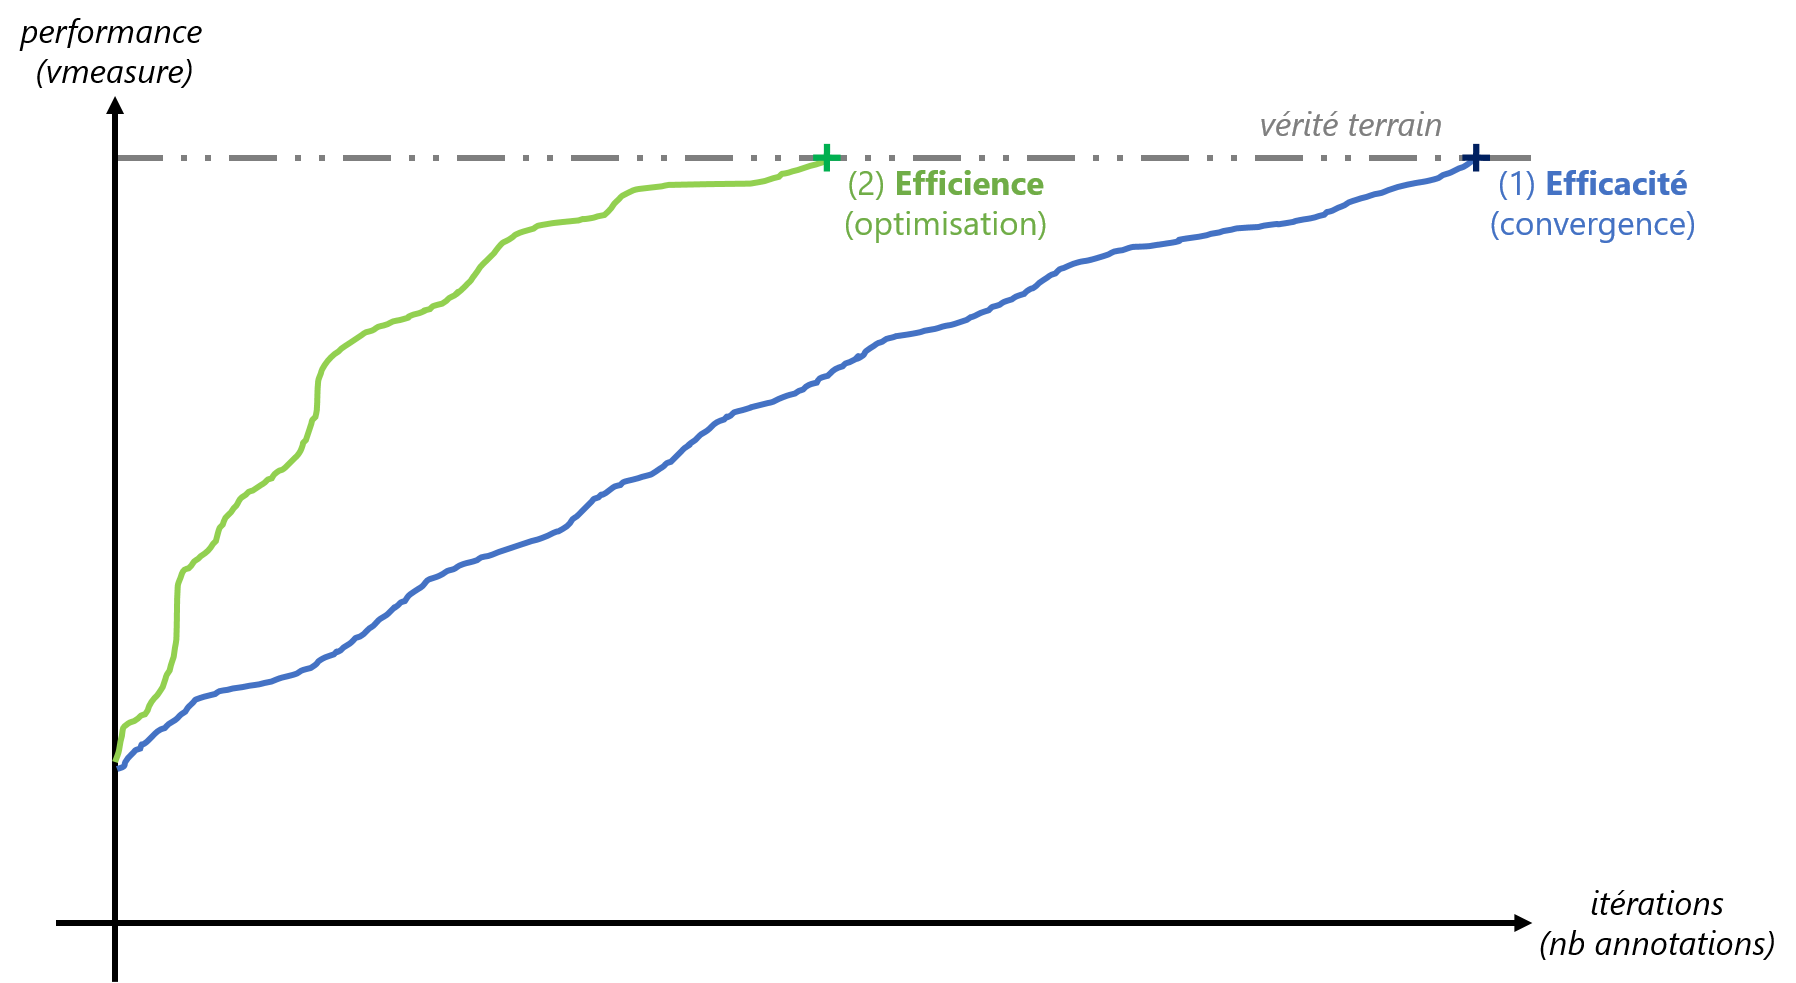
\includegraphics[width=0.8\textwidth]{figures/hypotheses-02-efficience}
				\caption{Illustration des études réalisées sur le \textit{clustering} interactif (\textit{étape 2/6}) en schématisant l'évolution de la performance (\textit{accord avec la vérité terrain calculé en v-measure}) d'une base d'apprentissage en cours de construction en fonction du nombre d'itérations de la méthode (\textit{nombre d'annotations par un expert métier}).}
				\label{figure:4.2-HYPOTHESE-EFFICIENCE}
			\end{figure}

		\end{tcolorbox}
		
		%%%
		%%% Subsection 4.2.1: Étude d'optimisation des paramètres de convergence.
		%%%
		\subsection{Étude d'optimisation des paramètres de convergence}
		\label{subsection:4.2.1-ETUDE-OPTIMISATION}
				
			% Référence articles.
			Cette étude a été l'objet d'une présentation à la conférence \texttt{EGC (Extraction et Gestion des Connaissances)}~\citep{schild:conception-interactive-clustering:2021}, et d'une extension dans le journal \texttt{IJDWM (International Journal of Data Warehousing and Mining)}~\citep{schild:extension-interactive-clustering:2022}.
	
			%%% Protocole expérimental.
			\subsubsection{Protocole expérimental : analyser la taille d'effet paramètres sur la vitesse de création d'une base d'apprentissage}

				% Objectif de l'expérience.
				Nous voulons étudier l'influence des paramètres de notre implémentation du \textit{clustering} interactif sur la vitesse de création d'une base d'apprentissage pour un assistant conversationnel.
				Pour cette étude, nous allons reprendre le protocole expérimental de l'étude de convergence en section~\ref{subsection:4.1.1-ETUDE-CONVERGENCE} visant à simuler la création d'une base d'apprentissage\todo{référence, lien vers ANNEXE}.
				
				% Détails de l'expérience.
				En s'appuyant sur les résultats précédemment obtenus, nous allons analyser l'influence des différentes tâches employées (\textbf{prétraitement}, \textbf{vectorisation}, \textbf{clustering sous contraintes}, \textbf{échantillonnage}) et de leurs paramètres sur la vitesse de convergence vers la vérité terrain.
				% Description implémentation de l'interactive clustering.
				Nous avons toujours 192 combinaisons testées, et chaque tentative est répétée 5 fois pour contrer les aléas statistiques de certains algorithmes.
				Pour plus de détails sur ces algorithmes, référez-vous à la section~\ref{section:3.3-DESCRIPTION-IMPLEMENTATION}.
				
				% Description de l'évaluation et Seuils d'évaluation.
				Comme lors de l'étude sur la convergence de la méthode, nous nous intéresserons à l'évolution de la \texttt{v-measure} entre la vérité terrain et notre segmentation des données obtenue, et nous affinerons notre évaluation en portant attentation aux trois seuils d'annotations suivants :
				\begin{enumerate}
					\item (\textbf{\textit{nouveau}}) le cas d'une \textbf{annotation partielle}, correspondant au nombre d'itérations nécessaires à la méthode pour avoir 80\% de \texttt{v-measure} entre le résultat obtenu et la vérité terrain, c'est-à-dire un état de semi-parcours vers une convergence totale\footnote{Le seuil de 80\% a été arbitrairement choisi pour cette étude.} ;\todo{pourquoi un nouveau seuil à 80\%}
					\item le cas d'une \textbf{annotation suffisante}, correspondant au nombre d'itérations nécessaires à la méthode pour avoir 100\% de \texttt{v-measure} entre le résultat obtenu et la vérité terrain, c'est-à-dire avoir suffisamment de contraintes annotées par l'expert métier pour retrouver la vérité terrain ;
					\item le cas d'une \textbf{annotation exhaustive}, correspondant au nombre d'itérations nécessaires à la méthode pour parcourir toutes les contraintes possibles sur les données, et ainsi retranscrire exhaustivement la vision de l'expert métier.
				\end{enumerate}
				
				% Description de l'analyse ANOVA.
				Enfin, nous utiliserons une \texttt{ANOVA} à mesures répétées afin de déterminer l’effet des paramètres de notre implémentation sur le nombre d’annotations requis pour converger vers la vérité terrain. Ces mesure seront réalisées à l’aide du logiciel R\todo{citation}, et les \texttt{Tukey HSD} est utilisé pour les comparaisons post-hoc.
				
				% Pseudo-code.
				Pour résumer ce protocole expérimental, vous pouvez vous référez au pseudo-code décrit dans Alg.~\ref{algorithm:4.2.1-ETUDE-OPTIMISATION-PROTOCOLE}.
				%
				\begin{algorithm}
					\begin{algorithmic}[1]
						\Require jeu de données annoté (vérité terrain)
						\ForAll{arrangement d'algorithmes et de paramètres à tester}
							\State \textbf{initialisation}: récupérer les données de la vérité terrain sans leur label, créer une liste vide de contraintes
							\State \textbf{prétraitement}: supprimer le bruit dans les données
							\State \textbf{vectorisation}: transformer les données en vecteurs
							\State \textbf{clustering initial}: regrouper les données par similarité
							\State \textbf{évaluation}: estimer l'équivalence entre le clustering obtenu et la vérité terrain
							\Repeat
								\State \textbf{échantillonnage}: sélectionner de nouvelles contraintes à annoter
								\State \textbf{simulation d'annotation}: ajouter des contraintes grâce à la comparaison des labels de la vérité terrain
								\State \textbf{clustering}: regrouper les données par similarité avec les contraintes
								\State \textbf{évaluation}: estimer l'équivalence entre le clustering obtenu et la vérité terrain
							\Until{annotation de toutes les contraintes possibles}
						\EndFor
						\State \textbf{analyse}: déterminer les tailles d'effets des algorithmes et paramètres
						\Ensure meilleurs arrangements d'algorithmes et de paramètres
					\end{algorithmic}
					\caption{Description en pseudo-code du protocole expérimental de l'étude d'optimisation de la convergence du \textit{clustering} interactif vers une vérité terrain pré-établie.}
					\label{algorithm:4.2.1-ETUDE-OPTIMISATION-PROTOCOLE}
				\end{algorithm}
				
				% Référence scripts.
				Les scripts de l'expérience (\textit{notebooks} Python) sont disponibles dans un dossier dédié de~\cite{schild:cognitivefactory-interactive-clustering-comparative-study:2021}.

			%%% Résultats
			\subsubsection{Résultats obtenus}
			
				% Analyse d'une annotation partielle.
				Le tableau~\ref{table:4.2.1-ETUDE-OPTIMISATION-ANOVA-ANNOTATION-PARTIELLE} retranscrit l'influence de chacun des paramètres sur le nombre d'itérations nécessaires pour atteindre une \textbf{annotation partielle} (\textit{atteindre une \texttt{v-measure} de 80\%}).
				Les analyses de variance mettent en relief l'effet significatif sur cette convergence du prétraitement (eta-carré: \texttt{0.992}, p-valeur: \(<\) \texttt{\(10^{-3}\)}), de la vectorisation (eta-carré: \texttt{0.998}, p-valeur: \(<\) \texttt{\(10^{-3}\)}), du clustering (eta-carré: \texttt{0.999}, p-valeur: \(<\) \texttt{\(10^{-3}\)}) et de l'échantillonnage (eta-carré: \texttt{0.999}, p-valeur: \(<\) \texttt{\(10^{-3}\)}).
				L'analyse post-hoc de ces effets indique que le meilleur paramétrage moyen pour atteindre une \textbf{annotation partielle} repose sur la prétraitement \texttt{prep.simple}, le vectorisation \texttt{vect.tfidf}, le clustering \texttt{clust.hier.avg} ou \texttt{clust.hier.sing}, et l'échantillonnage \texttt{samp.closest.diff}. La moyenne du nombre d'itération requis pour ce paramétrage est de \texttt{13.00} (écart-type: \texttt{2.11}), soit 650 annotations (écart-type: \texttt{105.50}).
				%
				\begin{table}[H]
					\begin{center}
					\begin{tabular}{|c|c|c|c|c|c|c|}
						\hline
						% ENTETE DU TABLEAU
						\multicolumn{2}{|c|}{ \shortstack{Description des \\ facteurs analysés } }
							& \multicolumn{3}{c|}{ \shortstack{ Description \\ statistique } }
							& \multicolumn{2}{c|}{ \shortstack{ Description des \\ tailles d'effets } }
							\tabularnewline
							\hline

						Facteur
							& Niveau 
							& Moyenne
							& Rang
							& SE
							& \texttt{ \( \eta^{2} \) }
							& \texttt{p-valeur}
						\tabularnewline
						\hline
						
						% PRETRAITEMENT
						\multirow{4}{*}{prétraitement}
							& \texttt{prep.simple}
							& \( 55.95 \)
							& (1)
							& \multirow{4}{*}{ \( 0.33 \) }
							& \multirow{4}{*}{ \( 0.992 \) }
							& \multirow{4}{*}{ \shortstack{ \( 7.72e^{-13} \) \\ (\( *** \)) } }
							\tabularnewline
							\cline{2-4}
							
							& \texttt{prep.lemma}
							& \( 57.25 \)
							& (2)
							&
							&
							&
							\tabularnewline
							\cline{2-4}
							
							& \texttt{prep.no}
							& \( 57.59 \)
							& (2)
							&
							& 
							&
							\tabularnewline
							\cline{2-4}
							
							& \texttt{prep.filter}
							& \( 65.36 \)
							& (4)
							&
							&
							&
							\tabularnewline
							\hline
						
						% VECTORISATION
						\multirow{2}{*}{vectorisation}
							& \texttt{vect.tfidf}
							& \( 55.00 \)
							& (1)
							& \multirow{2}{*}{ \( 0.30 \) }
							& \multirow{2}{*}{ \( 0.998 \) }
							& \multirow{2}{*}{ \shortstack{\( 1.56e^{-06} \) \\ (\( *** \)) } }
							\tabularnewline
							\cline{2-4}
							
							& \texttt{vect.frcorenewsmd}
							& \( 63.08 \)
							& (2)
							&
							&
							&
							\tabularnewline
							\hline
						
						% CLUSTERING
						\multirow{6}{*}{clustering}
							& \texttt{clust.hier.avg}
							& \( 44.89 \)
							& (1)
							& \multirow{6}{*}{ \( 0.32 \) }
							& \multirow{6}{*}{ \( 0.999 \) }
							& \multirow{6}{*}{ \shortstack{ \( < 2e^{-16} \) \\ (\( *** \)) } }
							\tabularnewline
							\cline{2-4}
							
							& \texttt{clust.hier.sing}
							& \( 45.27 \)
							& (1)
							&
							&
							&
							\tabularnewline
							\cline{2-4}
							
							& \texttt{clust.kmeans.cop}
							& \( 46.55 \)
							& (3)
							&
							& 
							&
							\tabularnewline
							\cline{2-4}
							
							& \texttt{clust.hier.ward}
							& \( 65.79 \)
							& (4)
							&
							& 
							&
							\tabularnewline
							\cline{2-4}
							
							& \texttt{clust.hier.comp}
							& \( 66.90 \)
							& (5)
							&
							&
							&
							\tabularnewline
							\cline{2-4}
							
							& \texttt{clust.spec}
							& \( 84.83 \)
							& (6)
							&
							& 
							&
							\tabularnewline
							\hline
						
						% ECHANTILLONNAGE
						\multirow{4}{*}{échantillonnage}
							& \texttt{samp.closest.diff}
							& \( 29.27 \)
							& (1)
							& \multirow{4}{*}{ \( 0.33 \) }
							& \multirow{4}{*}{ \( 0.999 \) }
							& \multirow{4}{*}{ \shortstack{ \( < 2e^{-16} \) \\ (\( *** \)) } }
							\tabularnewline
							\cline{2-4}
							
							& \texttt{samp.random.same}
							& \( 44.93 \)
							& (2)
							&
							&
							&
							\tabularnewline
							\cline{2-4}
							
							& \texttt{samp.random.full}
							& \( 61.07 \)
							& (3)
							&
							& 
							&
							\tabularnewline
							\cline{2-4}
							
							& \texttt{samp.farhtest.same}
							& \( 101.88 \)
							& (4)
							&
							&
							&
							\tabularnewline
							\hline
					\end{tabular}
					\end{center}
					\caption{ANOVA du nombre d'itérations nécessaires pour l'obtention de 80\% de V-mesure. Les (\textit{\(*\)}) dénotent le niveau de significativité (\(\alpha=0.05\)). Pour les effets significatifs, les chiffres précisés entre parenthèses dans la colonne \texttt{Moyenne} indiquent le classement des niveaux selon les analyses post-hoc.}
					\label{table:4.2.1-ETUDE-OPTIMISATION-ANOVA-ANNOTATION-PARTIELLE}
				\end{table}
				

			
				% Analyse d'une annotation suffisante.
				Le tableau~\ref{table:4.2.1-ETUDE-OPTIMISATION-ANOVA-ANNOTATION-SUFFISANTE} retranscrit l'influence de chacun des paramètres sur le nombre d'itérations nécessaires pour atteindre une \textbf{annotation suffisante} (\textit{atteindre une \texttt{v-measure} de 100\%}).
				Les analyses de variance mettent en relief l'effet significatif sur cette convergence du prétraitement (eta-carré: \texttt{0.987}, p-valeur: \(<\) \texttt{\(10^{-3}\)}), de la vectorisation (eta-carré: \texttt{0.991}, p-valeur: \(<\) \texttt{\(10^{-3}\)}), du clustering (eta-carré: \texttt{0.997}, p-valeur: \(<\) \texttt{\(10^{-3}\)}) et de l'échantillonnage (eta-carré: \texttt{0.998}, p-valeur: \(<\) \texttt{\(10^{-3}\)}).
				L'analyse post-hoc de ces effets indique que le meilleur paramétrage moyen pour atteindre une \textbf{annotation suffisante} repose sur la prétraitement \texttt{prep.lemma}, le vectorisation \texttt{vect.tfidf}, le clustering \texttt{clust.kmeans.cop}, et l'échantillonnage \texttt{samp.closest.diff}. La moyenne du nombre d'itération requis pour ce paramétrage est de \texttt{34.60} (écart-type: \texttt{7.44}), soit 1 730 annotations (écart-type: \texttt{372.00}).
				%
				\begin{table}[H]
					\begin{center}
					\begin{tabular}{|c|c|c|c|c|c|c|}
						\hline
						% ENTETE DU TABLEAU
						\multicolumn{2}{|c|}{ \shortstack{Description des \\ facteurs analysés } }
							& \multicolumn{3}{c|}{ \shortstack{ Description \\ statistique } }
							& \multicolumn{2}{c|}{ \shortstack{ Description des \\ tailles d'effets } }
							\tabularnewline
							\hline

						Facteur
							& Niveau 
							& Moyenne
							& Rang
							& SE
							& \texttt{ \( \eta^{2} \) }
							& \texttt{p-valeur}
						\tabularnewline
						\hline
						
						% PRETRAITEMENT
						\multirow{4}{*}{prétraitement}
							& \texttt{prep.lemma}
							& \( 72.86 \)
							& (1)
							& \multirow{4}{*}{ \( 0.32 \) }
							& \multirow{4}{*}{ \( 0.987 \) }
							& \multirow{4}{*}{ \shortstack{ \( 1.17e^{-13} \) \\ (\( *** \)) } }
							\tabularnewline
							\cline{2-4}
							
							& \texttt{prep.simple}
							& \( 73.30 \)
							& (2)
							&
							&
							&
							\tabularnewline
							\cline{2-4}
							
							& \texttt{prep.no}
							& \( 75.24 \)
							& (2)
							&
							& 
							&
							\tabularnewline
							\cline{2-4}
							
							& \texttt{prep.filter}
							& \( 83.77 \)
							& (4)
							&
							&
							&
							\tabularnewline
							\hline
						
						% VECTORISATION
						\multirow{2}{*}{vectorisation}
							& \texttt{vect.tfidf}
							& \( 71.16 \)
							& (1)
							& \multirow{2}{*}{ \( 0.36 \) }
							& \multirow{2}{*}{ \( 0.991 \) }
							& \multirow{2}{*}{ \shortstack{\( 9.30e^{-07} \) \\ (\( *** \)) } }
							\tabularnewline
							\cline{2-4}
							
							& \texttt{vect.frcorenewsmd}
							& \( 81.43 \)
							& (2)
							&
							&
							&
							\tabularnewline
							\hline
						
						% CLUSTERING
						\multirow{6}{*}{clustering}
							& \texttt{clust.kmeans.cop}
							& \( 62.23 \)
							& (1)
							& \multirow{6}{*}{ \( 0.42 \) }
							& \multirow{6}{*}{ \( 0.997 \) }
							& \multirow{6}{*}{ \shortstack{ \( < 2e^{-16} \) \\ (\( *** \)) } }
							\tabularnewline
							\cline{2-4}
							
							& \texttt{clust.hier.avg}
							& \( 65.13 \)
							& (2)
							&
							&
							&
							\tabularnewline
							\cline{2-4}
							
							& \texttt{clust.hier.sing}
							& \( 75.44 \)
							& (3)
							&
							& 
							&
							\tabularnewline
							\cline{2-4}
							
							& \texttt{clust.hier.ward}
							& \( 80.44 \)
							& (4)
							&
							& 
							&
							\tabularnewline
							\cline{2-4}
							
							& \texttt{clust.hier.comp}
							& \( 81.46 \)
							& (5)
							&
							&
							&
							\tabularnewline
							\cline{2-4}
							
							& \texttt{clust.spec}
							& \( 93.06 \)
							& (6)
							&
							& 
							&
							\tabularnewline
							\hline
						
						% ECHANTILLONNAGE
						\multirow{4}{*}{échantillonnage}
							& \texttt{samp.closest.diff}
							& \( 50.29 \)
							& (1)
							& \multirow{4}{*}{ \( 0.39 \) }
							& \multirow{4}{*}{ \( 0.998 \) }
							& \multirow{4}{*}{ \shortstack{ \( < 2e^{-16} \) \\ (\( *** \)) } }
							\tabularnewline
							\cline{2-4}
							
							& \texttt{samp.random.same}
							& \( 56.38 \)
							& (2)
							&
							&
							&
							\tabularnewline
							\cline{2-4}
							
							& \texttt{samp.random.full}
							& \( 71.95 \)
							& (3)
							&
							& 
							&
							\tabularnewline
							\cline{2-4}
							
							& \texttt{samp.farhtest.same}
							& \( 126.55 \)
							& (4)
							&
							&
							&
							\tabularnewline
							\hline
					\end{tabular}
					\end{center}
					\caption{ANOVA du nombre d'itérations nécessaires pour l'obtention de 100\% de V-mesure. Les (\textit{\(*\)}) dénotent le niveau de significativité (\(\alpha=0.05\)). Pour les effets significatifs, les chiffres précisés entre parenthèses dans la colonne \texttt{Moyenne} indiquent le classement des niveaux selon les analyses post-hoc.}
					\label{table:4.2.1-ETUDE-OPTIMISATION-ANOVA-ANNOTATION-SUFFISANTE}
				\end{table}
				
				
				% Analyse d'une annotation complète.
				Le tableau~\ref{table:4.2.1-ETUDE-OPTIMISATION-ANOVA-ANNOTATION-EXHAUSTIVE} retranscrit l'influence de chacun des paramètres sur le nombre d'itérations nécessaires pour atteindre une \textbf{annotation exhaustive} (\textit{annoter toutes les contraintes possibles}).
				Les analyses de variance mettent en relief l'effet significatif sur cette convergence du prétraitement (eta-carré: \texttt{0.909}, p-valeur: \(<\) \texttt{\(10^{-3}\)}), de la vectorisation (eta-carré: \texttt{0.985}, p-valeur: \(<\) \texttt{\(10^{-3}\)}), du clustering (eta-carré: \texttt{0.999}, p-valeur: \(<\) \texttt{\(10^{-3}\)}) et de l'échantillonnage (eta-carré: \texttt{0.997}, p-valeur: \(<\) \texttt{\(10^{-3}\)}).
				L'analyse post-hoc de ces effets indique que le meilleur paramétrage moyen pour atteindre une \textbf{annotation exhaustive} repose sur la prétraitement \texttt{prep.lemma}, le vectorisation \texttt{vect.tfidf}, le clustering \texttt{clust.kmeans.cop}, et l'échantillonnage \texttt{samp.random.same}. La moyenne du nombre d'itération requis pour ce paramétrage est de \texttt{32.60} (écart-type: \texttt{1.14}), soit 1 630 annotations (écart-type: \texttt{57.00}).
				%
				\begin{table}[H]
					\begin{center}
					\begin{tabular}{|c|c|c|c|c|c|c|}
						\hline
						% ENTETE DU TABLEAU
						\multicolumn{2}{|c|}{ \shortstack{Description des \\ facteurs analysés } }
							& \multicolumn{3}{c|}{ \shortstack{ Description \\ statistique } }
							& \multicolumn{2}{c|}{ \shortstack{ Description des \\ tailles d'effets } }
							\tabularnewline
							\hline

						Facteur
							& Niveau 
							& Moyenne
							& Rang
							& SE
							& \texttt{ \( \eta^{2} \) }
							& \texttt{p-valeur}
						\tabularnewline
						\hline
						
						% PRETRAITEMENT
						\multirow{4}{*}{prétraitement}
							& \texttt{prep.lemma}
							& \( 85.89 \)
							& (1)
							& \multirow{4}{*}{ \( 0.42 \) }
							& \multirow{4}{*}{ \( 0.909 \) }
							& \multirow{4}{*}{ \shortstack{ \( 1.10e^{-08} \) \\ (\( *** \)) } }
							\tabularnewline
							\cline{2-4}
							
							& \texttt{prep.filter}
							& \( 89.55 \)
							& (2)
							&
							&
							&
							\tabularnewline
							\cline{2-4}
							
							& \texttt{prep.simple}
							& \( 89.64 \)
							& (2)
							&
							& 
							&
							\tabularnewline
							\cline{2-4}
							
							& \texttt{prep.no}
							& \( 90.81 \)
							& (4)
							&
							&
							&
							\tabularnewline
							\hline
						
						% VECTORISATION
						\multirow{2}{*}{vectorisation}
							& \texttt{vect.tfidf}
							& \( 85.50 \)
							& (1)
							& \multirow{2}{*}{ \( 0.39 \) }
							& \multirow{2}{*}{ \( 0.985 \) }
							& \multirow{2}{*}{ \shortstack{\( 2.53e^{-06} \) \\ (\( *** \)) } }
							\tabularnewline
							\cline{2-4}
							
							& \texttt{vect.frcorenewsmd}
							& \( 92.46 \)
							& (2)
							&
							&
							&
							\tabularnewline
							\hline
						
						% CLUSTERING
						\multirow{6}{*}{clustering}
							& \texttt{clust.kmeans.cop}
							& \( 64.99 \)
							& (1)
							& \multirow{6}{*}{ \( 0.39 \) }
							& \multirow{6}{*}{ \( 0.999 \) }
							& \multirow{6}{*}{ \shortstack{ \( < 2e^{-16} \) \\ (\( *** \)) } }
							\tabularnewline
							\cline{2-4}
							
							& \texttt{clust.hier.avg}
							& \( 78.54 \)
							& (2)
							&
							&
							&
							\tabularnewline
							\cline{2-4}
							
							& \texttt{clust.hier.ward}
							& \( 81.31 \)
							& (3)
							&
							& 
							&
							\tabularnewline
							\cline{2-4}
							
							& \texttt{clust.hier.comp}
							& \( 82.49 \)
							& (3)
							&
							& 
							&
							\tabularnewline
							\cline{2-4}
							
							& \texttt{clust.spec}
							& \( 93.78 \)
							& (5)
							&
							&
							&
							\tabularnewline
							\cline{2-4}
							
							& \texttt{clust.hier.comp}
							& \( 132.75 \)
							& (6)
							&
							& 
							&
							\tabularnewline
							\hline
						
						% ECHANTILLONNAGE
						\multirow{4}{*}{échantillonnage}
							& \texttt{samp.random.same}
							& \( 57.23 \)
							& (1)
							& \multirow{4}{*}{ \( 0.42 \) }
							& \multirow{4}{*}{ \( 0.997 \) }
							& \multirow{4}{*}{ \shortstack{ \( < 2e^{-16} \) \\ (\( *** \)) } }
							\tabularnewline
							\cline{2-4}
							
							& \texttt{samp.random.full}
							& \( 72.80 \)
							& (2)
							&
							&
							&
							\tabularnewline
							\cline{2-4}
							
							& \texttt{samp.closest.diff}
							& \( 98.38 \)
							& (3)
							&
							& 
							&
							\tabularnewline
							\cline{2-4}
							
							& \texttt{samp.farhtest.same}
							& \( 132.75 \)
							& (4)
							&
							&
							&
							\tabularnewline
							\hline
					\end{tabular}
					\end{center}
					\caption{ANOVA du nombre d'itérations nécessaires pour annoter toutes les contraintes possibles. Les (\textit{\(*\)}) dénotent le niveau de significativité (\(\alpha=0.05\)). Pour les effets significatifs, les chiffres précisés entre parenthèses dans la colonne \texttt{Moyenne} indiquent le classement des niveaux selon les analyses post-hoc.}
					\label{table:4.2.1-ETUDE-OPTIMISATION-ANOVA-ANNOTATION-EXHAUSTIVE}
				\end{table}
			
			
				% Graphe d'évolution de la v-measure moyenne, min et max.
				La figure~\ref{figure:4.2.1-ETUDE-CONVERGENCE-EVOLUTION-PAR-FACTEURS} représente les évolutions moyennes de la \texttt{v-measure} du clustering en fonction du nombre d'itération de la méthode pour les différentes valeurs des facteurs analysés (prétraitement en haut à gauche, vectorisation en haut à droite, clustering en bas à gauche, échantillonnage en bas à droite).
				%
				\begin{figure}[H]
					\centering
					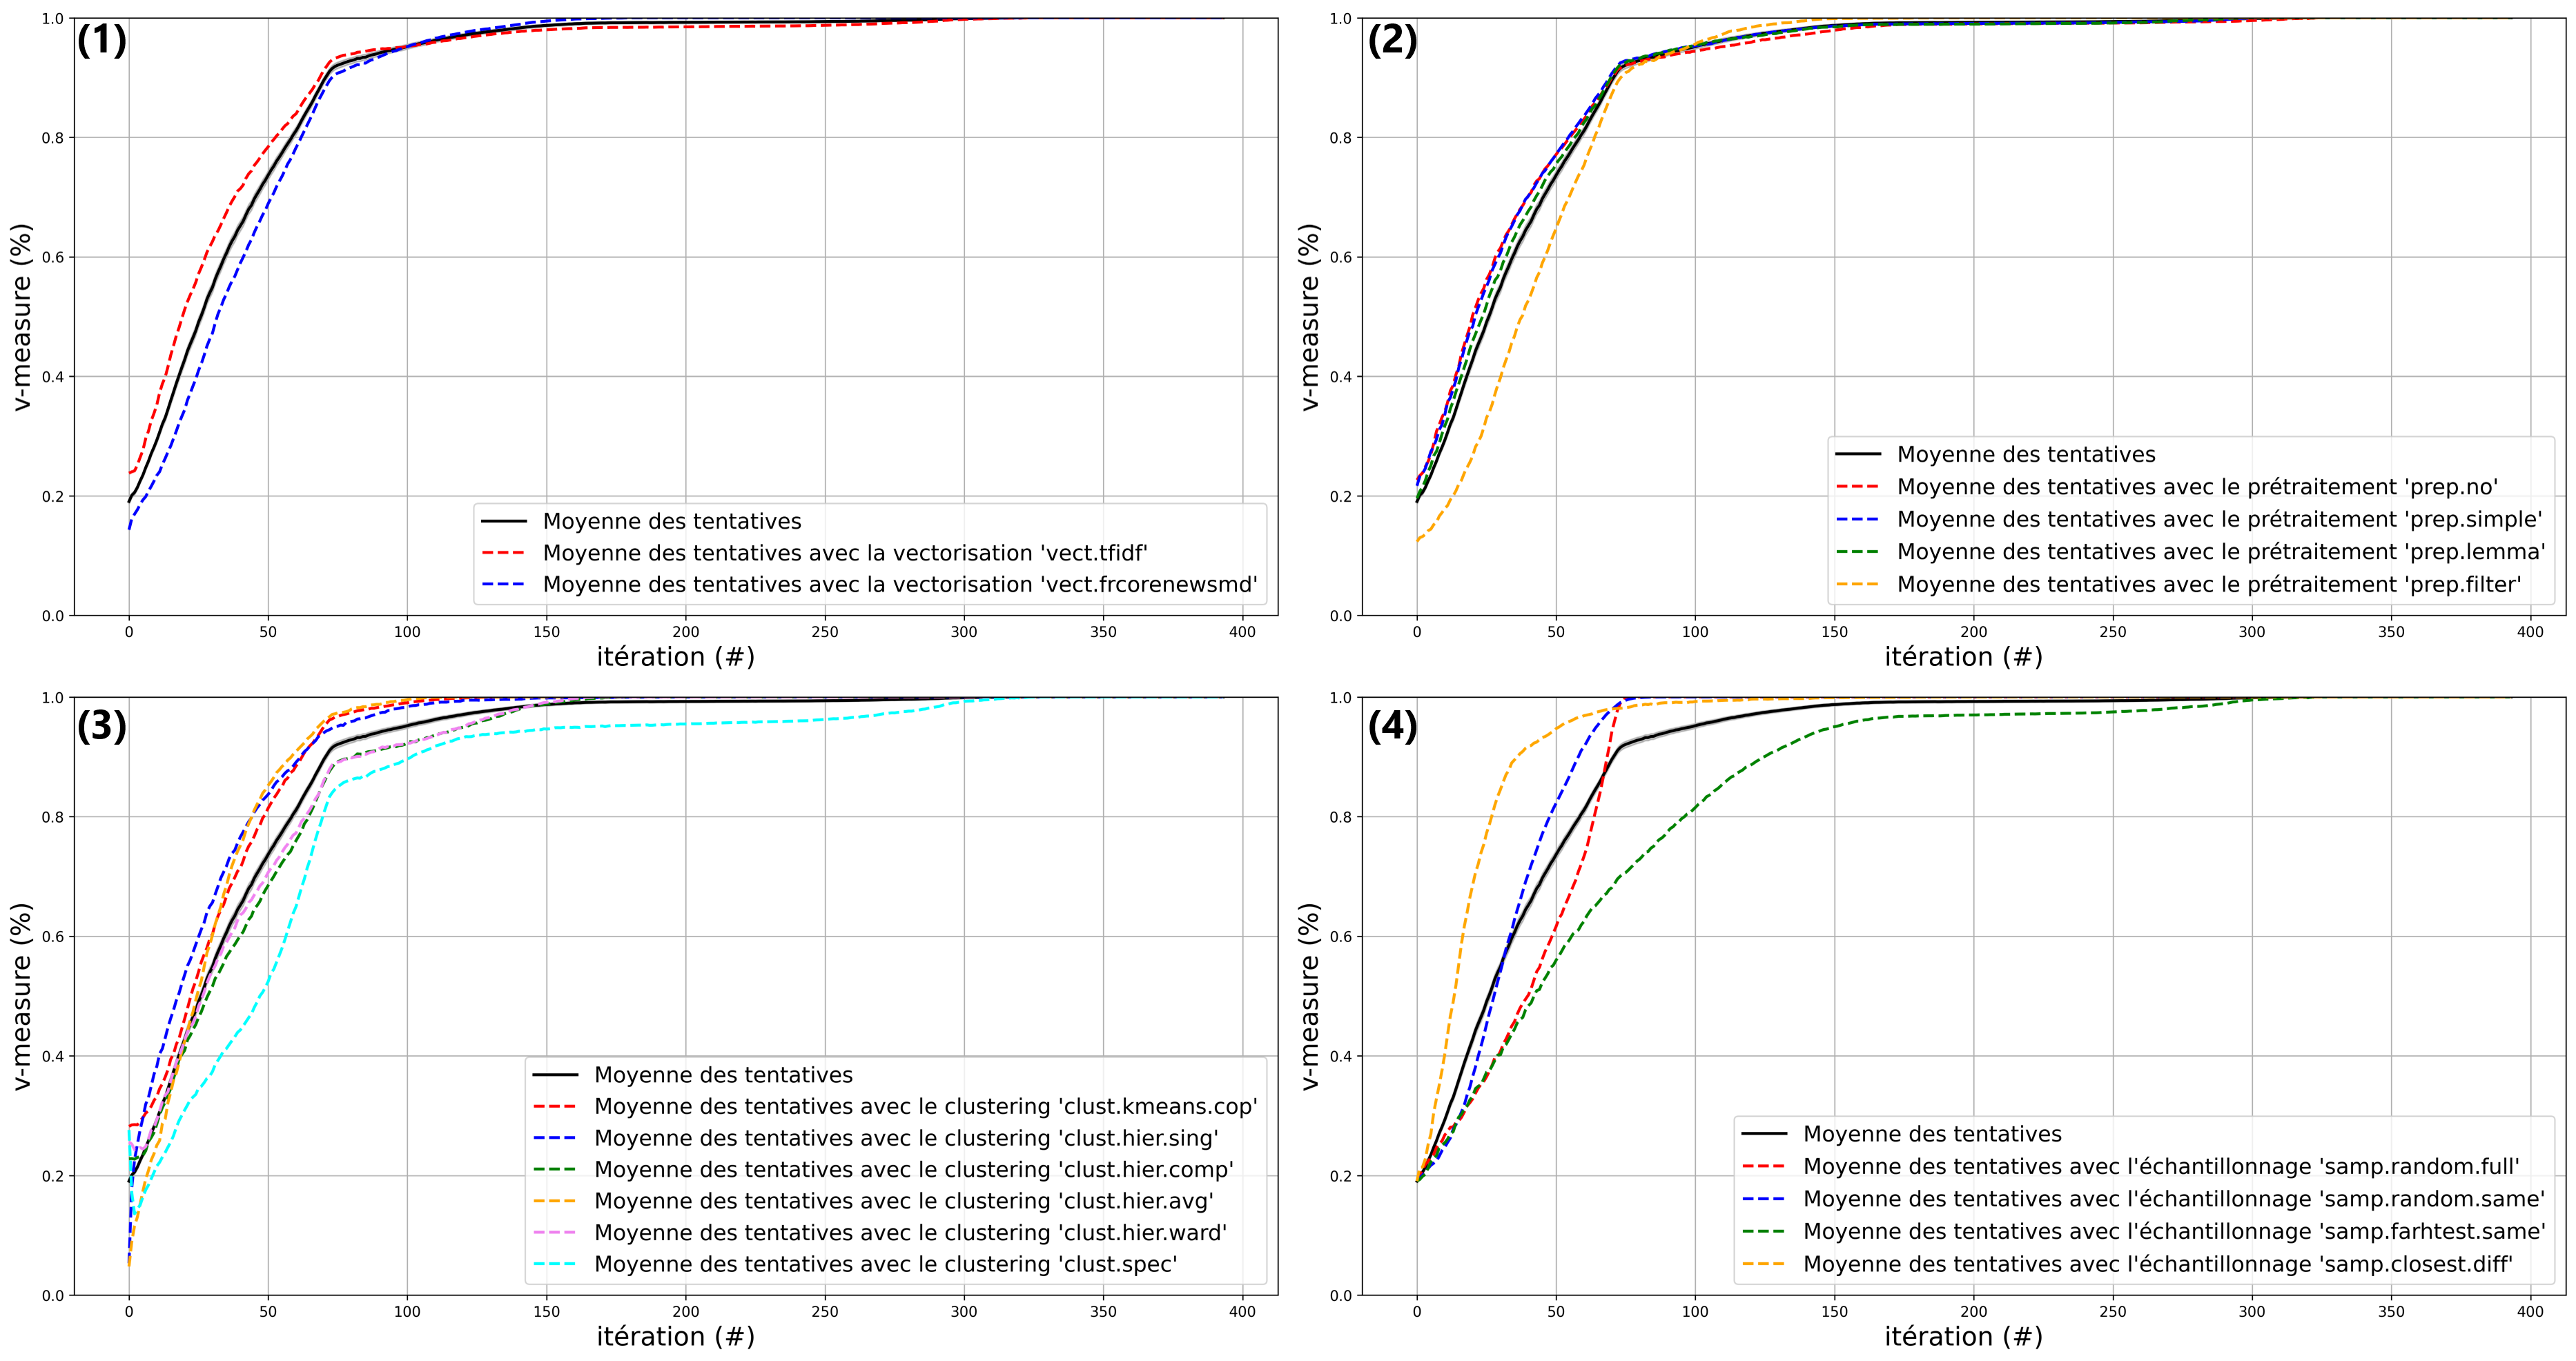
\includegraphics[width=0.8\textwidth]{figures/etude-convergence-evolution-moyenne-par-iteration-par-facteur}
					\caption{Évolution des moyennes de la \texttt{v-measure} entre un résultat obtenu et la vérité terrain en fonction du nombre d'itération de la méthode de \textit{clustering} interactif, moyennes réalisées itération par itération sur les différentes valeurs que peuvent prendre les facteurs analysés et affichées par facteur : \textbf{(1)} prétraitement, \textbf{(2)} vectorisation, \textbf{(3)} clustering et \textbf{(4)} échantillonnage.}
					\label{figure:4.2.1-ETUDE-CONVERGENCE-EVOLUTION-PAR-FACTEURS}
				\end{figure}

			%%% Discussion
			\subsubsection{Discussion}
				\todo{meilleur paramétrage}
	

    %%%%%--------------------------------------------------------------------
    %%%%% Section 4.3: Hypothèse de pertinence.
    %%%%%--------------------------------------------------------------------
    \section{Hypothèse de pertinence : « \textit{est-ce le résultat est exploitable ?} »}
	\label{section:4.3-HYPOTHESE-PERTINENCE}
	
		%%% Formulation des hypothèses:
		Nous aimerions vérifier l'hypothèse suivante :
		\todo{à compléter}

		\begin{tcolorbox}[
			title=\textbf{Hypothèse de pertinence},
			colback=gray!20,
			colframe=gray!50!black!75,
			width=\linewidth
		]
			« La vitesse de convergence du \textit{clustering} interactif \textbf{peut être optimisée} en réglant différents paramètres. Nous étudierons l'influence du prétraitement des données, de la vectorisation des données, de l'échantillonnage des contraintes à annoter et du \textit{clustering} sous contraintes (cf. figure~\ref{figure:HYPOTHESE-PERTINENCE}. »
			
			
			\begin{figure}[H]
				\centering
				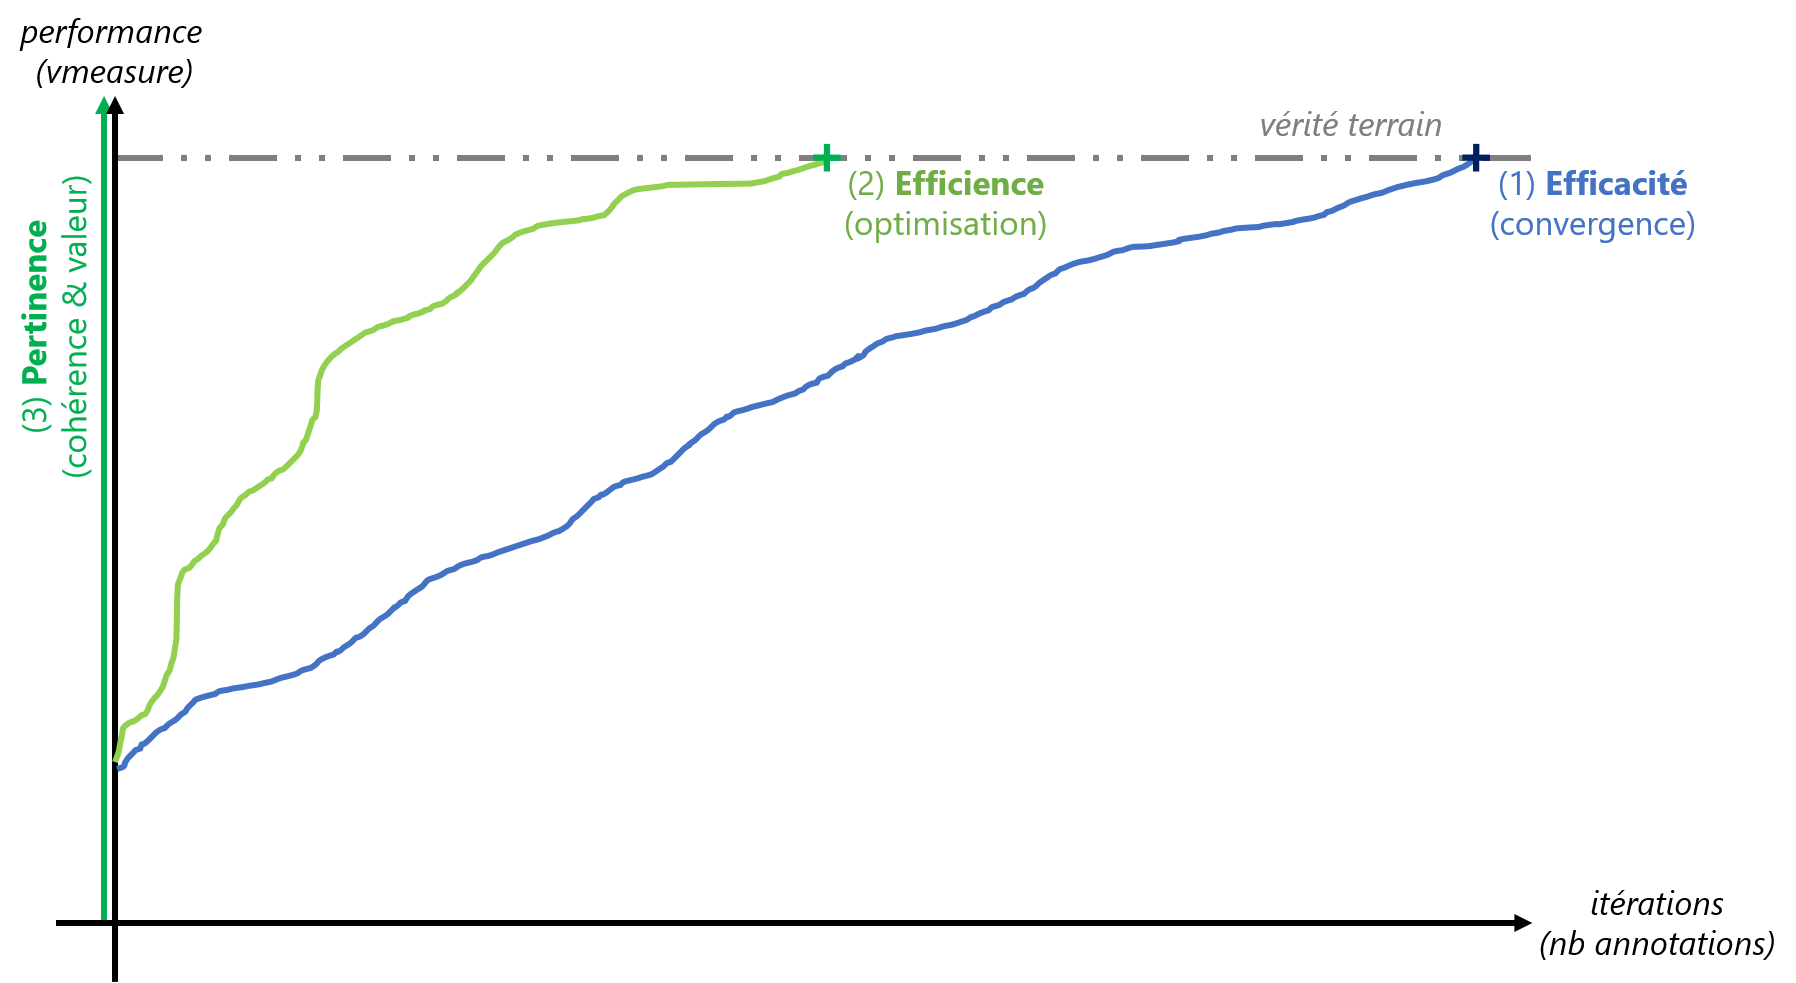
\includegraphics[width=0.8\textwidth]{figures/hypotheses-03-pertinence}
				\caption{Illustration des études réalisées sur le \textit{clustering} interactif (\textit{étape 3/6}) en schématisant l'évolution de la performance (\textit{accord avec la vérité terrain calculé en v-measure}) d'une base d'apprentissage en cours de construction en fonction du nombre d'itérations de la méthode (\textit{nombre d'annotations par un expert métier}).}
				\label{figure:HYPOTHESE-PERTINENCE}
			\end{figure}

		\end{tcolorbox}
		
		%%%
		%%% Subsection 4.3.1: Étude de la cohérence statistique de la base d'apprentissage en cours de construction
		%%%
		\subsection{Étude de la cohérence statistique de la base d'apprentissage en cours de construction}
		
			%%% Protocole expérimental.
			\subsubsection{Protocole expérimental}
				\todo[inline]{Description succincte du protocole expérimental dans l'encadré d'hypothèse ?}

			%%% Résultats
			\subsubsection{Résultats obtenus}

			%%% Discussion
			\subsubsection{Discussion}
		
		%%%
		%%% Subsection 4.3.2: Étude de la pertinence sémentique de la base d'apprentissage en cours de construction
		%%%
		\subsection{Étude de la pertinence sémentique de la base d'apprentissage en cours de construction}
		
			%%% Protocole expérimental.
			\subsubsection{Protocole expérimental}
				\todo[inline]{Description succincte du protocole expérimental dans l'encadré d'hypothèse ?}

			%%% Résultats
			\subsubsection{Résultats obtenus}

			%%% Discussion
			\subsubsection{Discussion}
	

    %%%%%--------------------------------------------------------------------
    %%%%% Section 4.4: Hypothèse sur les coûts.
    %%%%%--------------------------------------------------------------------
    \section{Hypothèse sur les coûts : « \textit{combien dois-je investir ?} »}
	\label{section:4.4-HYPOTHESE-COUTS}
	
		%%% Formulation des hypothèses:
		Nous aimerions vérifier l'hypothèse suivante :
		\todo{à compléter}

		\begin{tcolorbox}[
			title=\textbf{Hypothèse sur les coûts},
			colback=gray!20,
			colframe=gray!50!black!75,
			width=\linewidth
		]
			« Il est possible de \textbf{mesurer le temps nécessaire} à une méthodologie d'annotation basée sur le \textit{clustering} interactif pour obtenir un résultat exploitable (cf. figure~\ref{figure:HYPOTHESE-COUTS}. »
			
			
			\begin{figure}[H]
				\centering
				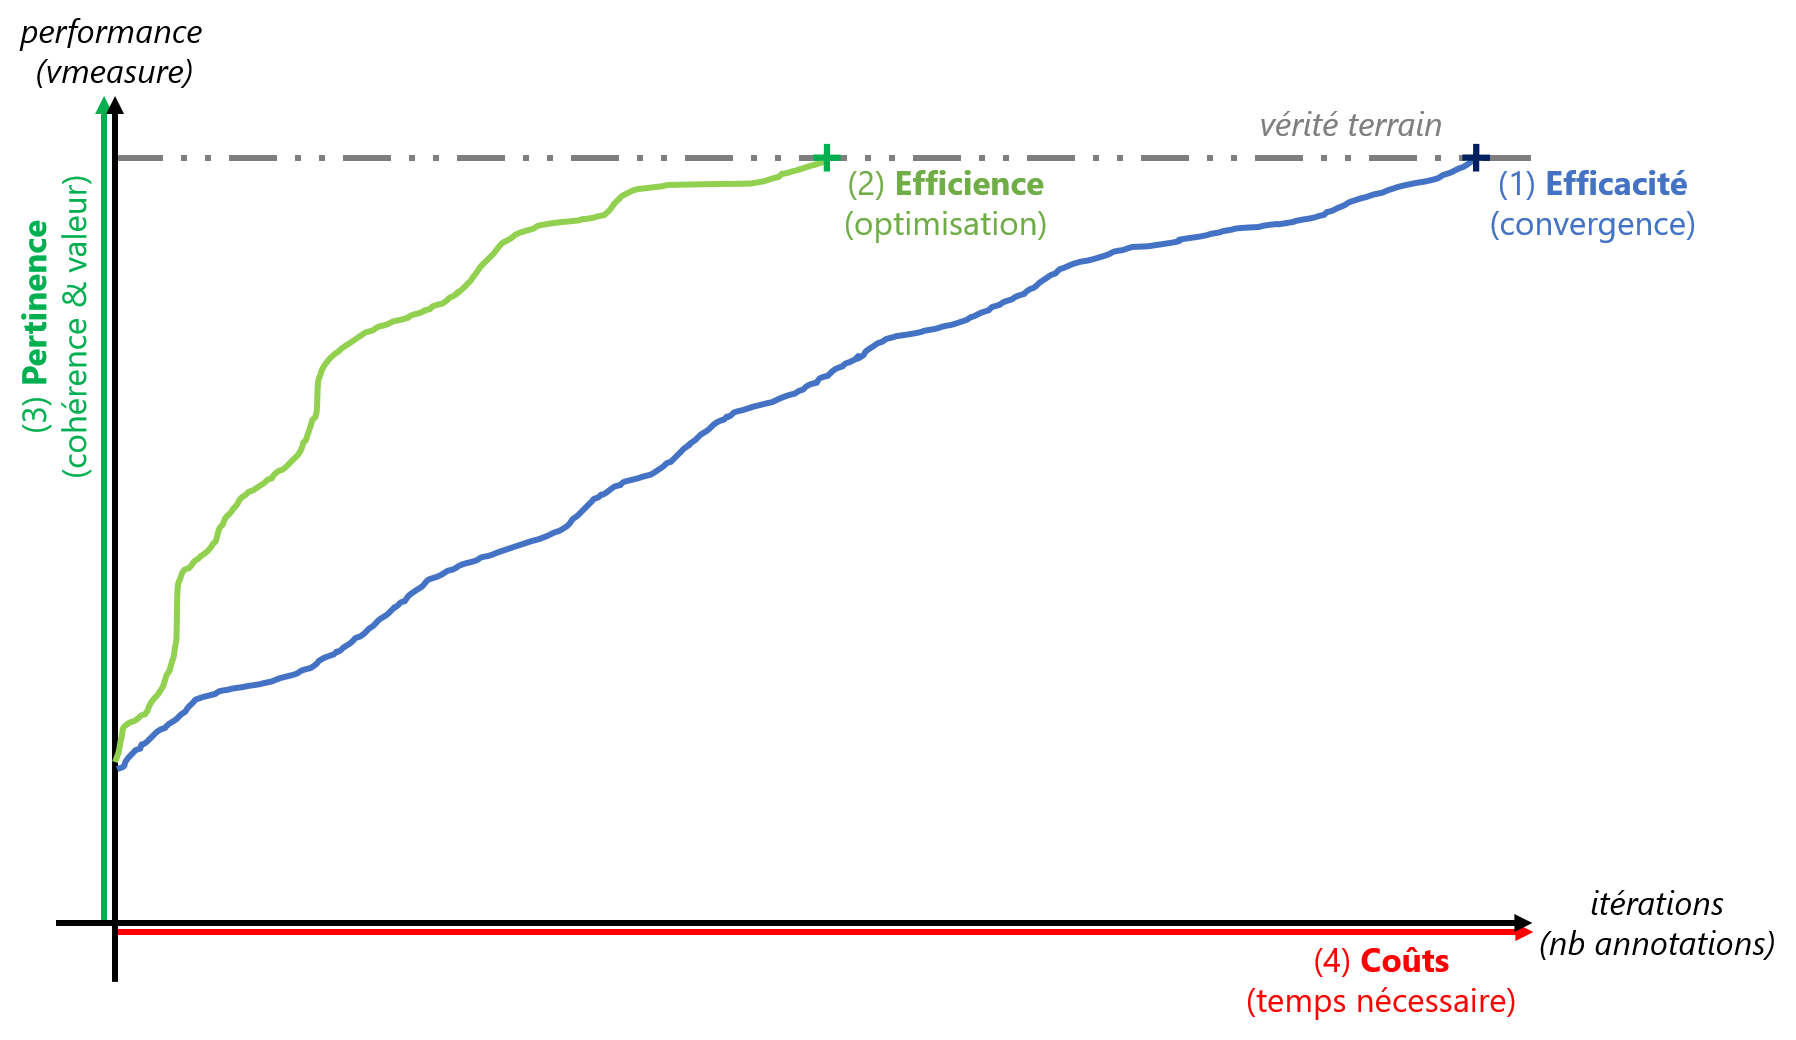
\includegraphics[width=0.8\textwidth]{figures/hypotheses-04-couts}
				\caption{Illustration des études réalisées sur le \textit{clustering} interactif (\textit{étape 4/6}) en schématisant l'évolution de la performance (\textit{accord avec la vérité terrain calculé en v-measure}) d'une base d'apprentissage en cours de construction en fonction du nombre d'itérations de la méthode (\textit{nombre d'annotations par un expert métier}).}
				\label{figure:HYPOTHESE-COUTS}
			\end{figure}

		\end{tcolorbox}
		
		%%%
		%%% Subsection 4.4.1: Étude d'estimation du temps d'annotation par un expert métier
		%%%
		\subsection{Étude d'estimation du temps d'annotation par un expert métier}
		
			%%% Protocole expérimental.
			\subsubsection{Protocole expérimental}
				\todo[inline]{Description succincte du protocole expérimental dans l'encadré d'hypothèse ?}

			%%% Résultats
			\subsubsection{Résultats obtenus}

			%%% Discussion
			\subsubsection{Discussion}
		
		%%%
		%%% Subsection 4.4.2: Étude d'estimation du temps de calcul des algorithmes
		%%%
		\subsection{Étude d'estimation du temps de calcul des algorithmes}
		
			%%% Protocole expérimental.
			\subsubsection{Protocole expérimental}
				\todo[inline]{Description succincte du protocole expérimental dans l'encadré d'hypothèse ?}

			%%% Résultats
			\subsubsection{Résultats obtenus}

			%%% Discussion
			\subsubsection{Discussion}
		
		%%%
		%%% Subsection 4.4.3: Étude d'estimation du temps total d'un projet d'annotation
		%%%
		\subsection{Étude d'estimation du temps total d'un projet d'annotation}
		
			%%% Protocole expérimental.
			\subsubsection{Protocole expérimental}
				\todo[inline]{Description succincte du protocole expérimental dans l'encadré d'hypothèse ?}

			%%% Résultats
			\subsubsection{Résultats obtenus}

			%%% Discussion
			\subsubsection{Discussion}
	

    %%%%%--------------------------------------------------------------------
    %%%%% Section 4.5: Hypothèse d'impact.
    %%%%%--------------------------------------------------------------------
    \section{Hypothèse d'impact : « \textit{quel gain à chaque itération ?} »}
	\label{section:4.5-HYPOTHESE-IMPACT}
	
		%%% Formulation des hypothèses:
		Nous aimerions vérifier l'hypothèse suivante :
		\todo{à reformuler}

		\begin{tcolorbox}[
			title=\textbf{Hypothèse d'impact},
			colback=gray!20,
			colframe=gray!50!black!75,
			width=\linewidth
		]
			« Il est possible d'estimer quand méthodologie d'annotation basée sur le \textit{clustering} interactif \textbf{a converger} vers un résultat satisfaisant (cf. figure~\ref{figure:HYPOTHESE-IMPACT}. »
			
			
			\begin{figure}[H]
				\centering
				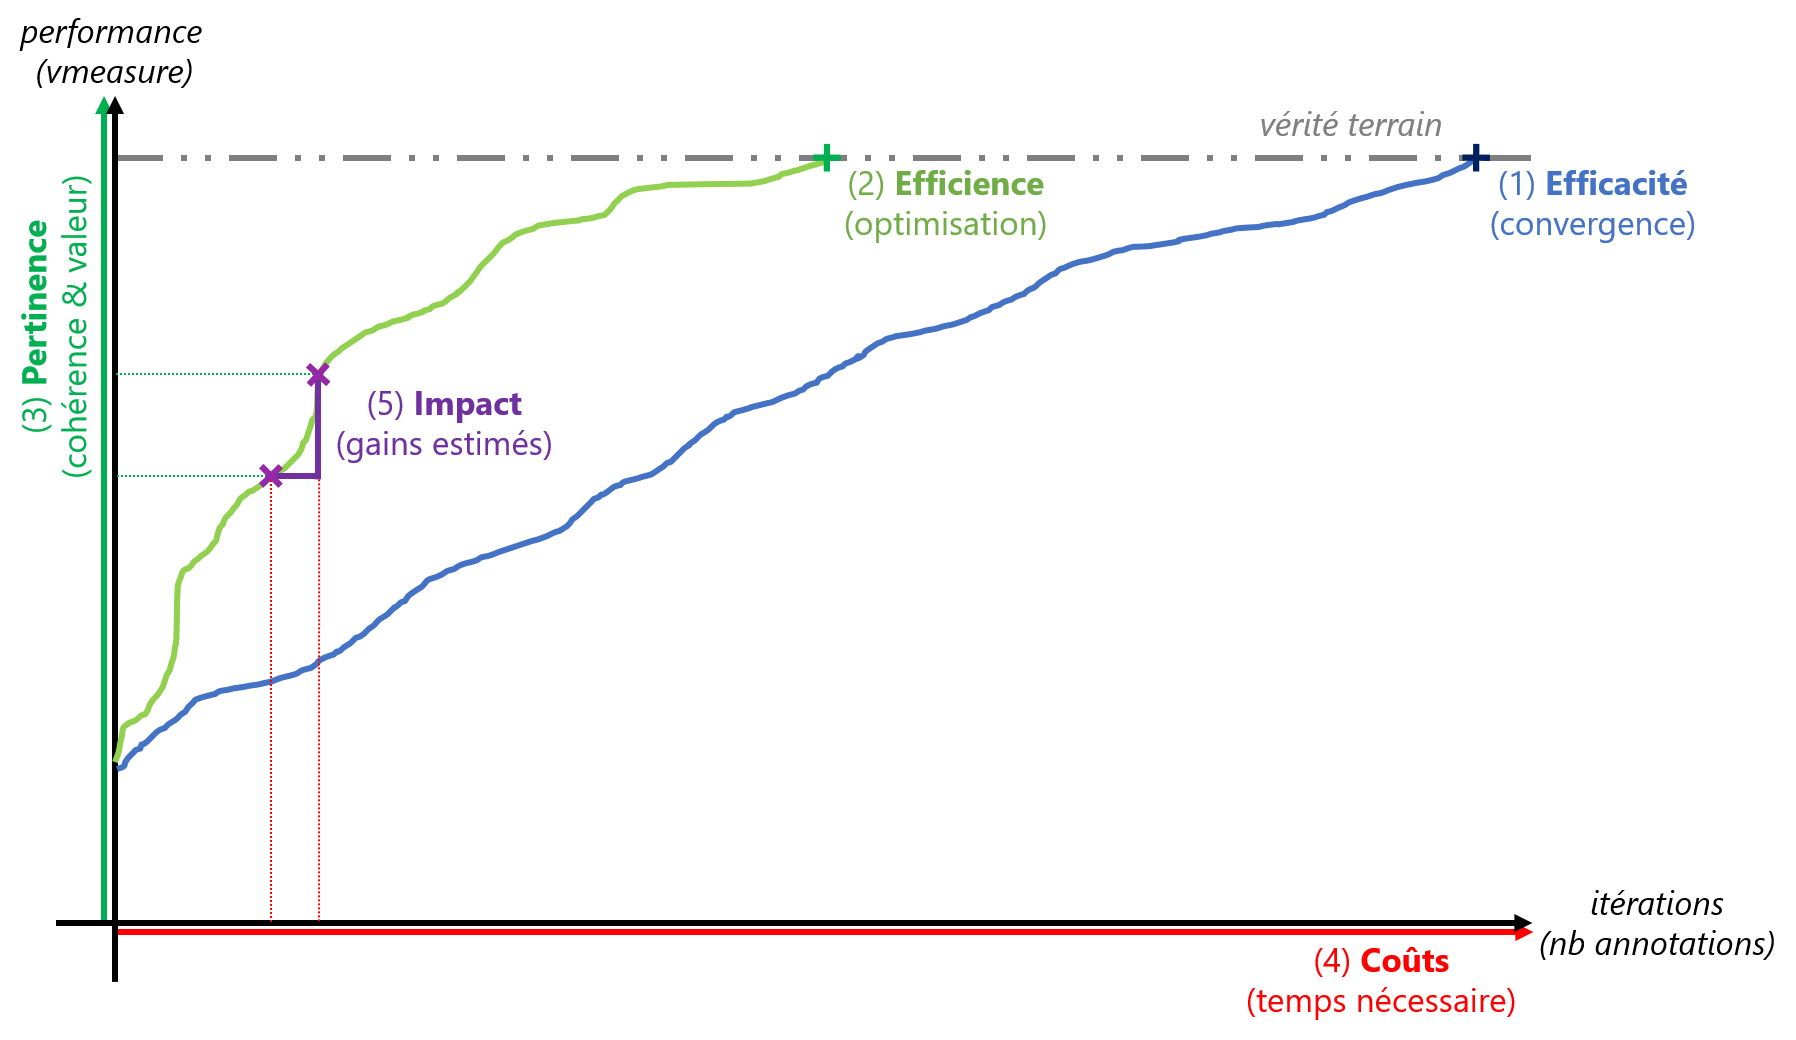
\includegraphics[width=0.8\textwidth]{figures/hypotheses-05-impact}
				\caption{Illustration des études réalisées sur le \textit{clustering} interactif (\textit{étape 5/6}) en schématisant l'évolution de la performance (\textit{accord avec la vérité terrain calculé en v-measure}) d'une base d'apprentissage en cours de construction en fonction du nombre d'itérations de la méthode (\textit{nombre d'annotations par un expert métier}).}
				\label{figure:HYPOTHESE-IMPACT}
			\end{figure}

		\end{tcolorbox}
		
		%%%
		%%% Subsection 4.5.1: Étude d'estimation des cas d'arrêts de la méthode
		%%%
		\subsection{Étude d'estimation des cas d'arrêts de la méthode}
		
			%%% Protocole expérimental.
			\subsubsection{Protocole expérimental}
				\todo[inline]{Description succincte du protocole expérimental dans l'encadré d'hypothèse ?}

			%%% Résultats
			\subsubsection{Résultats obtenus}

			%%% Discussion
			\subsubsection{Discussion}
	

    %%%%%--------------------------------------------------------------------
    %%%%% Section 4.6: Hypothèse de robustesse.
    %%%%%--------------------------------------------------------------------
    \section{Hypothèse de robustesse : « \textit{quelle influence d'une erreur ?} »}
	\label{section:4.6-HYPOTHESE-ROBUSTESSE}
	
		%%% Formulation des hypothèses:
		Nous aimerions vérifier l'hypothèse suivante :
		\todo{à reformuler}

		\begin{tcolorbox}[
			title=\textbf{Hypothèse de robustesse},
			colback=gray!20,
			colframe=gray!50!black!75,
			width=\linewidth
		]
			« Il est possible d'\textbf{estimer l'influence d'une différence d'annotation} lors d'une méthodologie d'annotation basée sur le \textit{clustering} interactif (cf. figure~\ref{figure:HYPOTHESE-ROBUSTESSE}. »
			
			
			\begin{figure}[H]
				\centering
				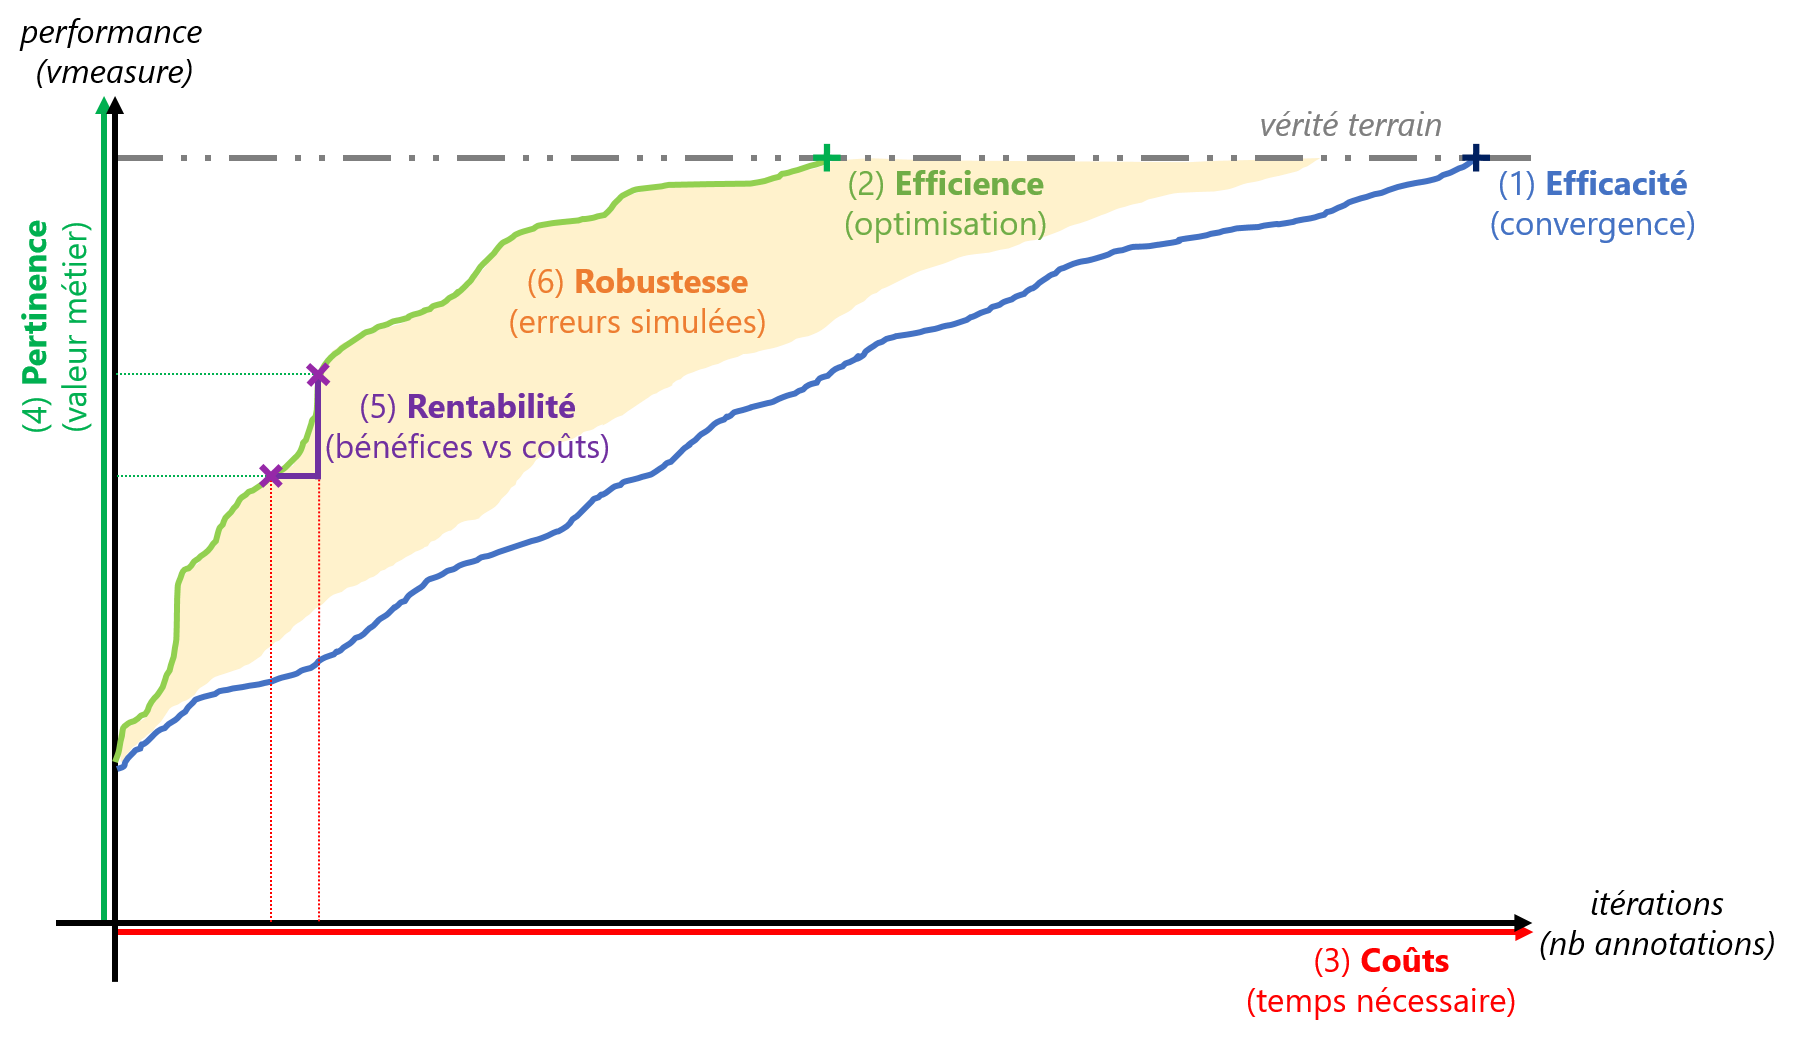
\includegraphics[width=0.8\textwidth]{figures/hypotheses-06-robustesse}
				\caption{Illustration des études réalisées sur le \textit{clustering} interactif (\textit{étape 6/6}) en schématisant l'évolution de la performance (\textit{accord avec la vérité terrain calculé en v-measure}) d'une base d'apprentissage en cours de construction en fonction du nombre d'itérations de la méthode (\textit{nombre d'annotations par un expert métier}).}
				\label{figure:HYPOTHESE-ROBUSTESSE}
			\end{figure}

		\end{tcolorbox}
		
		%%%
		%%% Subsection 4.6.1: Étude de simulation d'erreurs d'annotations
		%%%
		\subsection{Étude de simulation d'erreurs d'annotations}
		
			%%% Protocole expérimental.
			\subsubsection{Protocole expérimental}
				\todo[inline]{Description succincte du protocole expérimental dans l'encadré d'hypothèse ?}

			%%% Résultats
			\subsubsection{Résultats obtenus}

			%%% Discussion
			\subsubsection{Discussion}
		
		%%%
		%%% Subsection 4.6.2: Étude d'annotation avec des paradigmes différents
		%%%
		\subsection{Étude d'annotation avec des paradigmes différents}
		
			%%% Protocole expérimental.
			\subsubsection{Protocole expérimental}
				\todo[inline]{Description succincte du protocole expérimental dans l'encadré d'hypothèse ?}

			%%% Résultats
			\subsubsection{Résultats obtenus}

			%%% Discussion
			\subsubsection{Discussion}
			
	
    %%%%%--------------------------------------------------------------------
    %%%%% Section 4.7:
    %%%%%--------------------------------------------------------------------
    \section{Autres études à réaliser}
	\label{section:4.7-ETUDES-DIVERSES}
	\todo[inline]{SECTION À RÉDIGER}

        \subsection{Choix du nombre de clusters ==> problème de recherche complexe}
            o	Piste de résolution : plusieurs clusterings + vote collaboratif ? algorithmes sans le nombre de clusters en hyper-paramètres

        \subsection{Impact d'un modèle de langage ==> nécessite de nombreuses données spécifiques au domaine}
            o	Piste de résolution : script d'étude comparative déjà prêt, mais il manque les données opensources… 

        \subsection{Paradigme d’annotation (intention vs dialogue) ==> problème d'UX + objectif métier}
            o	Etude Ergo, sort de mon domaine d'expertise

        \subsection{(et plein d'autres que j'ajouterai au fur et à mesure de ma rédaction)}
            o	
